\chapter{External Specification}
\label{chap:external-specifications}

This chapter provides a detailed overview of the external specifications for the application. It outlines the specific requirements for its operation and the installation procedures necessary for a straightforward setup. Additionally, it includes key information to improve user understanding and ensure the application fulfils its intended purpose effectively.

\section{Hardware and Software Requirements}
\subsection{Hardware Requirements}
\begin{itemize}
    \item Android smartphone with Android 11.0 (API level 30) or higher.
    \item Camera with support for CameraX.
     \item Minimum 2GB RAM for standard use of the application, or 3GB RAM for optimal performance on devices with lower memory and processing power.
    \item Internet connection for the dice recognition module; the other parts of the app do not require internet and will work otherwise.
    \item At least 100MB of free storage space.
    \item Processor: ARM-based processor supporting Neon instruction set.
\end{itemize}

\subsection{Software Requirements}
This section outlines the essential software tools and dependencies required for the development and execution of the application. Ensuring compatibility with these components is crucial for the stability and performance of the system.
\begin{itemize}
    \item Android Studio Giraffe (2023.1.1) or later.
    \item Kotlin 2.0.21.
    \item Gradle 8.10.2 and the corresponding Android Gradle Plugin (e.g. 8.1.2).
    \item CameraX library version: 1.4.0.
\end{itemize}


\section{Installation Procedure}
This section details the necessary steps for installing and running the application on an Android device. Users must follow these instructions to ensure proper functionality and security.

\subsection{APK Download}
\begin{enumerate}
    \item Download the Release APK from the project's repository at \href{https://github.com/Mayokun-Sofowora/kavi/releases/download/v1.0.0/app-release.apk}{GitHub Releases Page}.
    \item Enable installation from unknown sources in the device's settings. Note that installing apps from unknown sources has security implications; please proceed with caution.
    \item Open the APK file and follow the on-screen instructions.
\end{enumerate}

\subsection{Building with Android Studio}
To install the application for debugging purposes, follow these steps:

\begin{enumerate}
    \item \textbf{Clone the Repository}: Start by cloning the project repository from GitHub.
    \begin{verbatim}
git clone https://github.com/Mayokun-Sofowora/kavi.git
    \end{verbatim}

    \item \textbf{Open in Android Studio}: Launch Android Studio and open the cloned project.

    \item  \textbf{API setup}: To use the dice recognition feature, the Roboflow API key must be configured. This section provides the necessary steps to obtain and configure the API key.
    \begin{itemize}
        \item Sign in to \href{https://roboflow.com/}{Roboflow}.
        \item Navigate to your Project Dashboard.
        \item Locate the API Key under the "Settings" or "Security" section.
        \item Add the api key to the \texttt{local.properties} file:
        \begin{verbatim}
    ROBOFLOW_API_KEY=api_key
        \end{verbatim}
    \end{itemize}

    \item \textbf{Sync Gradle Dependencies}: Allow Android Studio to sync the Gradle dependencies automatically.

    \item \textbf{Run on a Device or Emulator}: Connect an Android device or start an emulator with a minimum SDK version of 30, then run the application.
\end{enumerate}


In addition to the instructions provided, be sure that:
\begin{itemize}
    \item  A debug build variant is selected in Android Studio.
    \item USB debugging is enabled in the device's settings.
    \item You connect an Android device via USB or use an emulator.
    \item  You select the appropriate run configuration in Android Studio.
\end{itemize}

\section{Types of Users}
\begin{itemize}
    \item \textbf{Regular Users}: Play dice games, use image recognition features, and adjust settings.
    \item \textbf{Developers/Testers}: Access debugging logs, experimental features, and perform system administration tasks.
\end{itemize}

\section{User Manual}
\label{sec:user_manual}

\subsection{Navigating the App}

When starting the game, users are welcomed with a splash screen that displays the application's logo in Figure~\ref{fig:splash_screen}. After a short moment, the main menu is shown in Figure~\ref{fig:main_menu}. The main menu provides navigation options to access the different features of the application.
\begin{figure}[ht!]
    \centering
    \begin{subfigure}[b]{0.27\textwidth}
        \centering
        \fbox{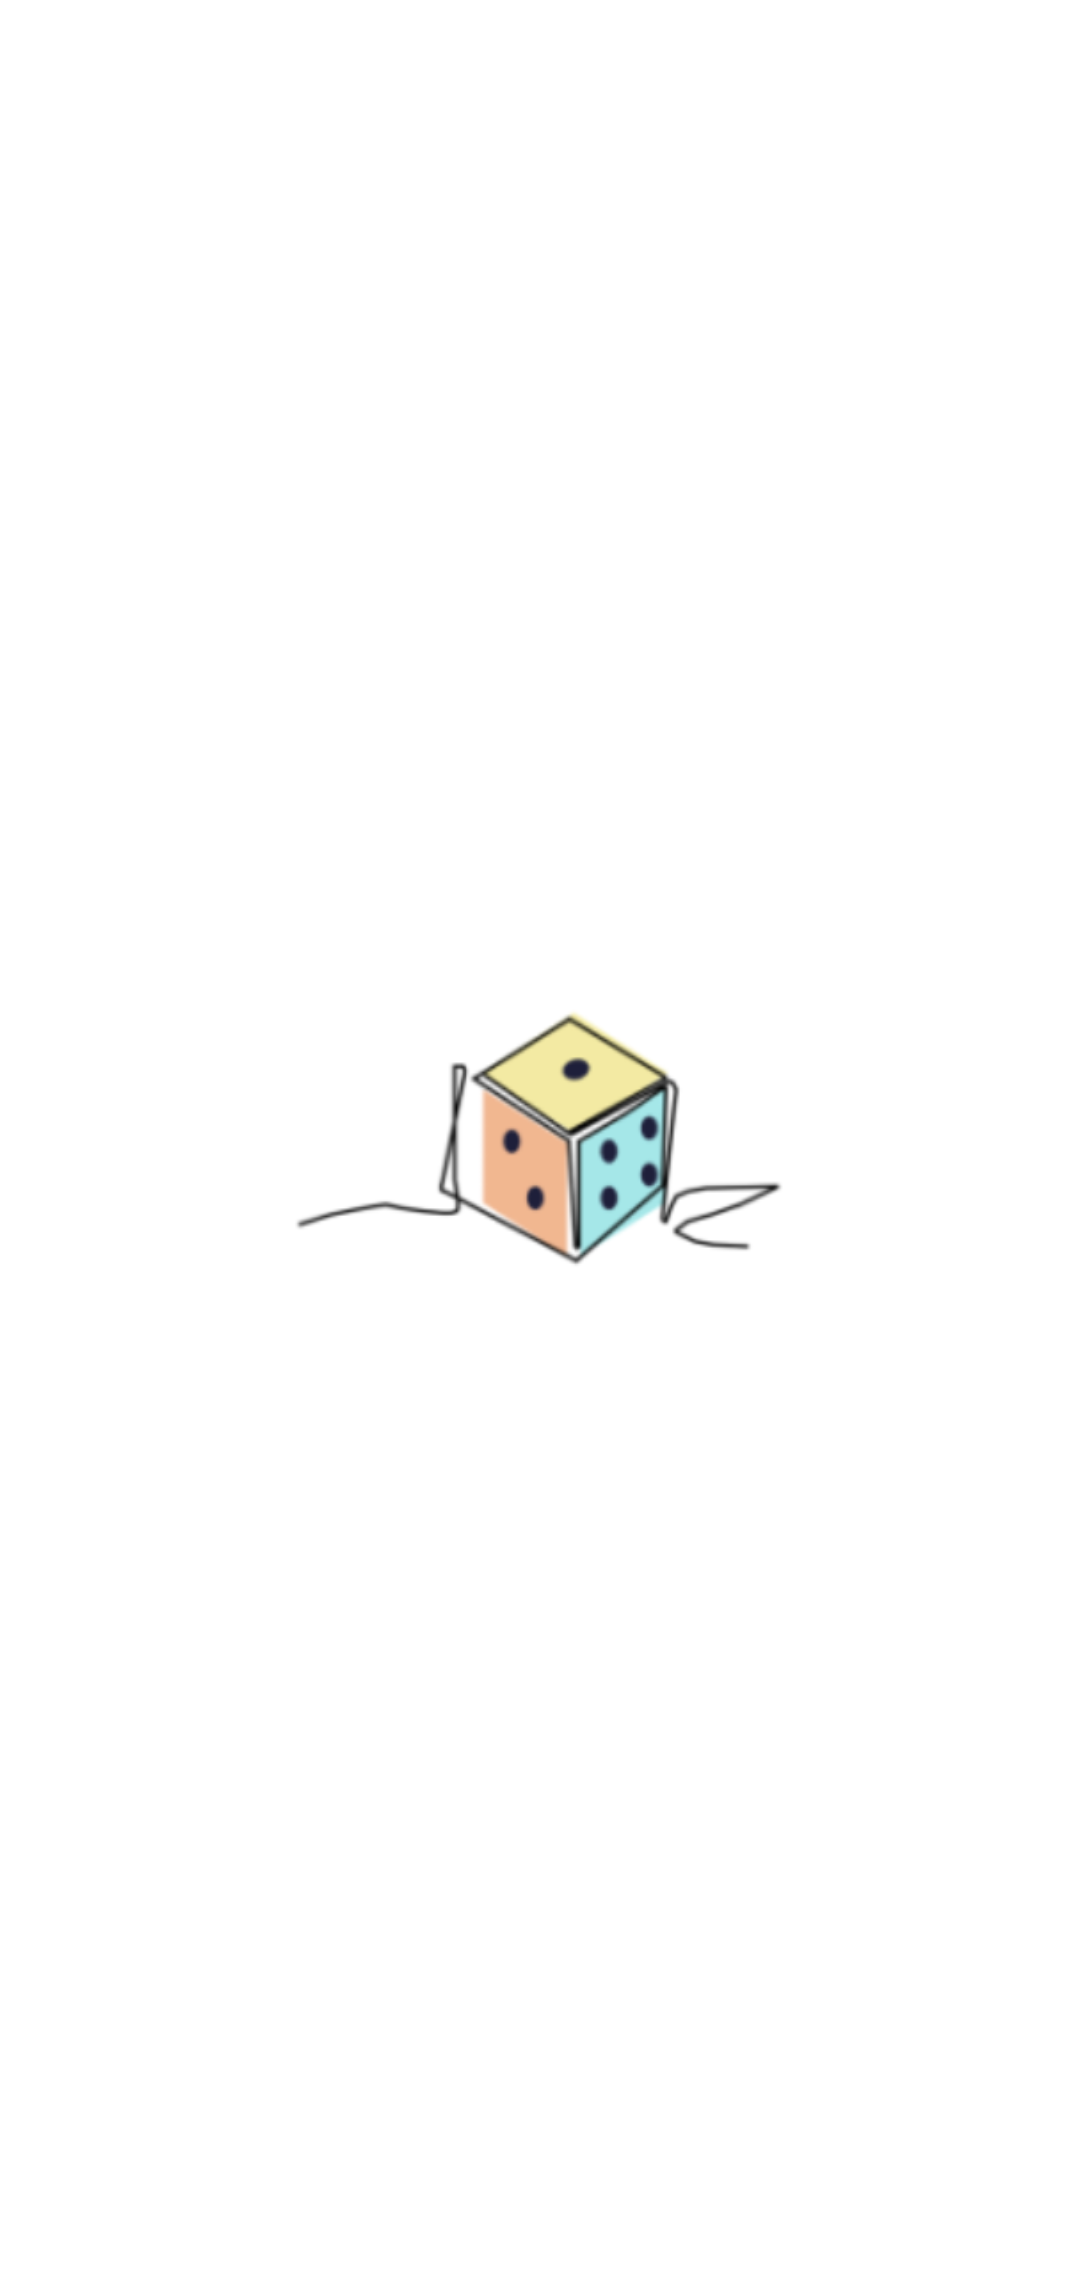
\includegraphics[width=\textwidth]{img/splash screen.png}}
        \caption{The Splash Screen}
        \label{fig:splash_screen}
    \end{subfigure}
    \hspace{1em}
    \begin{subfigure}[b]{0.27\textwidth}
        \centering
        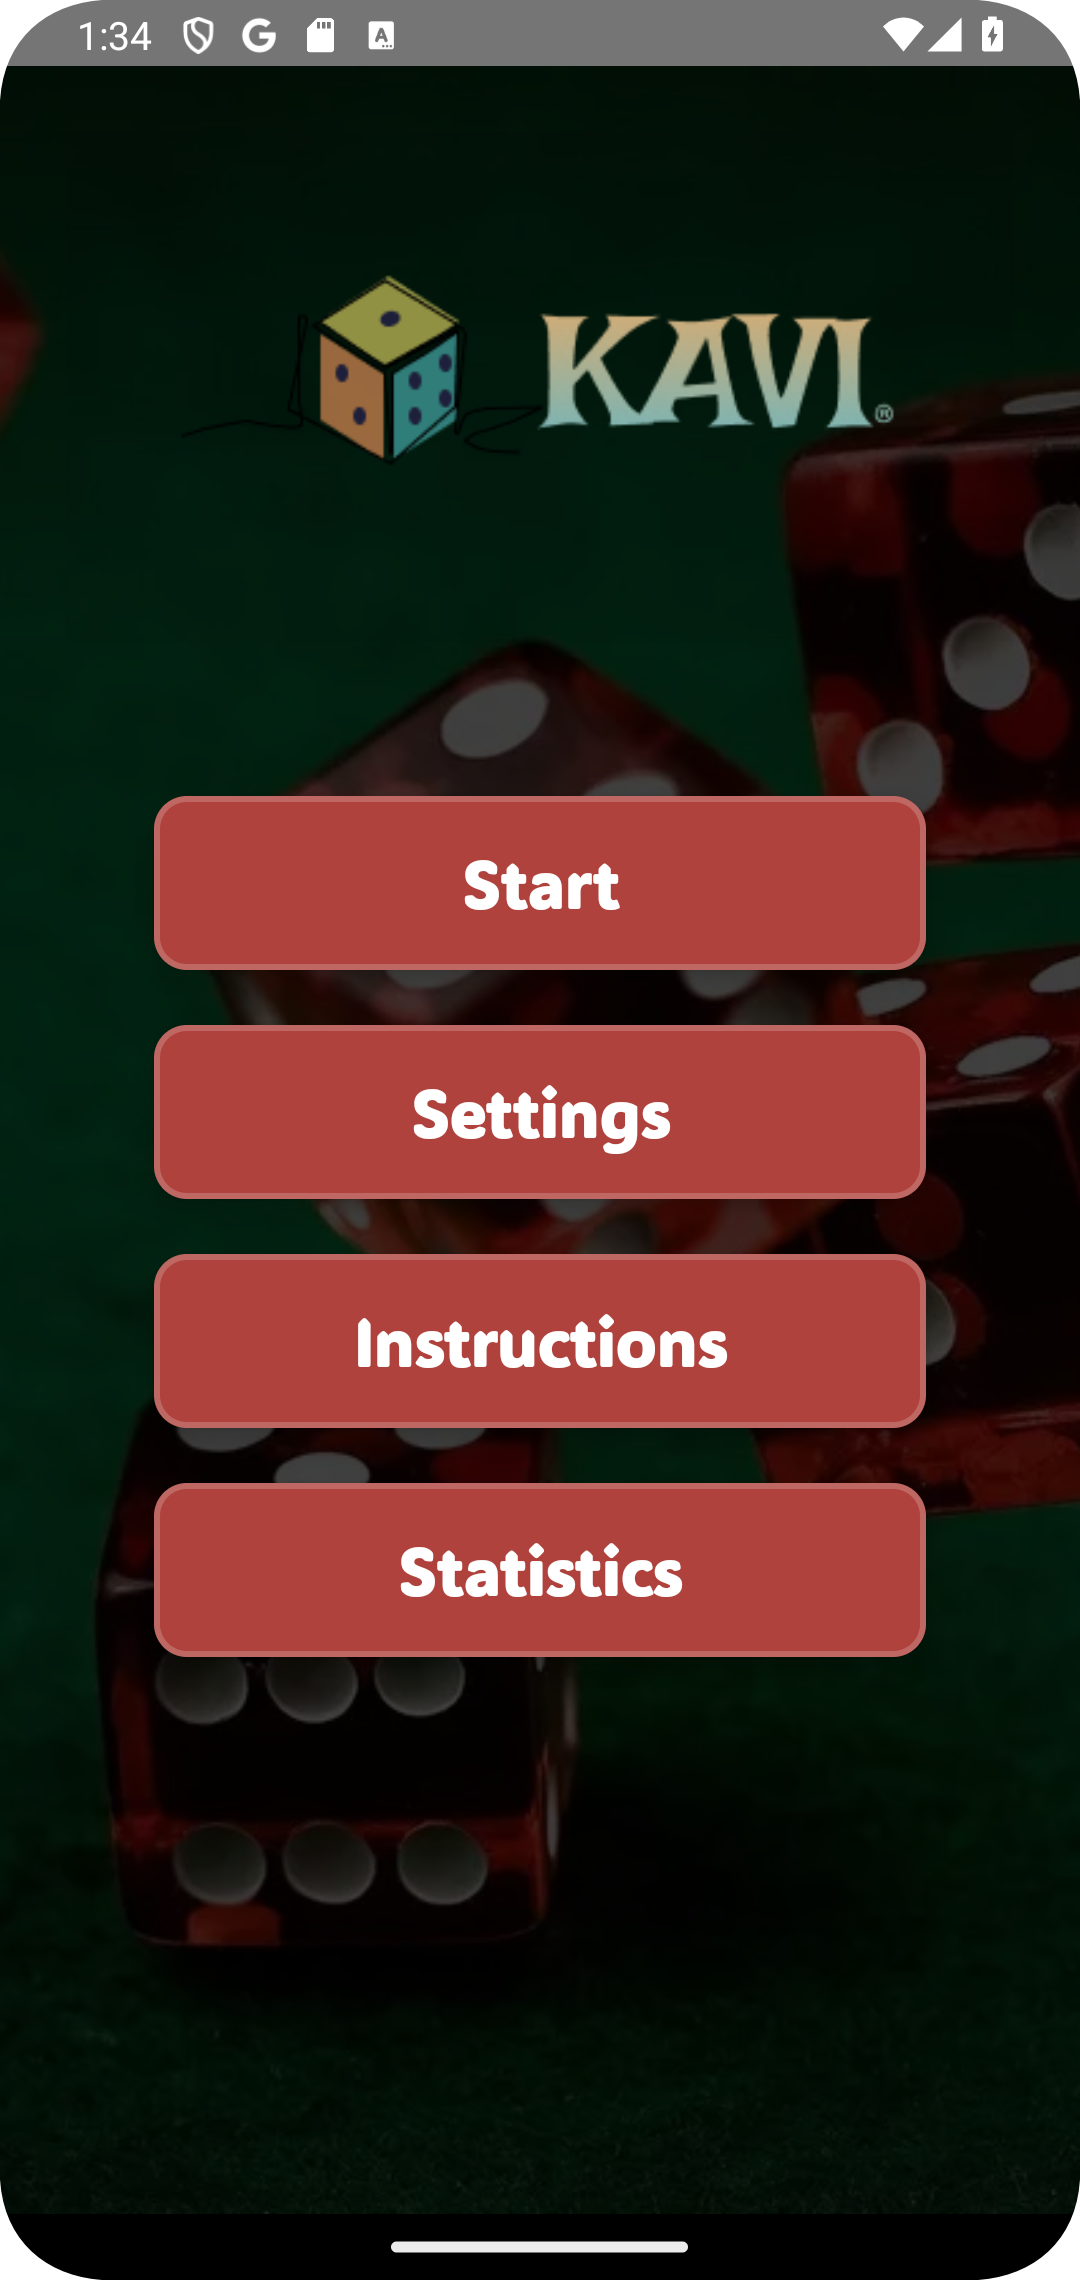
\includegraphics[width=\textwidth]{img/main menu.png}
        \caption{The Main Menu}
        \label{fig:main_menu}
    \end{subfigure}
    \caption{Screens displayed when starting the game.}
    \label{fig:starting_game}
\end{figure}

\subsection{Game Interface}

The interface allows users to navigate to different sections of the application, such as the classic boards to play the classic dice games or the virtual screen to use the image recognition feature. The Figure~\ref{fig:interface_mode} shows the navigation options available.

\begin{figure}[ht!]
    \centering
    \begin{subfigure}[b]{0.27\textwidth}
        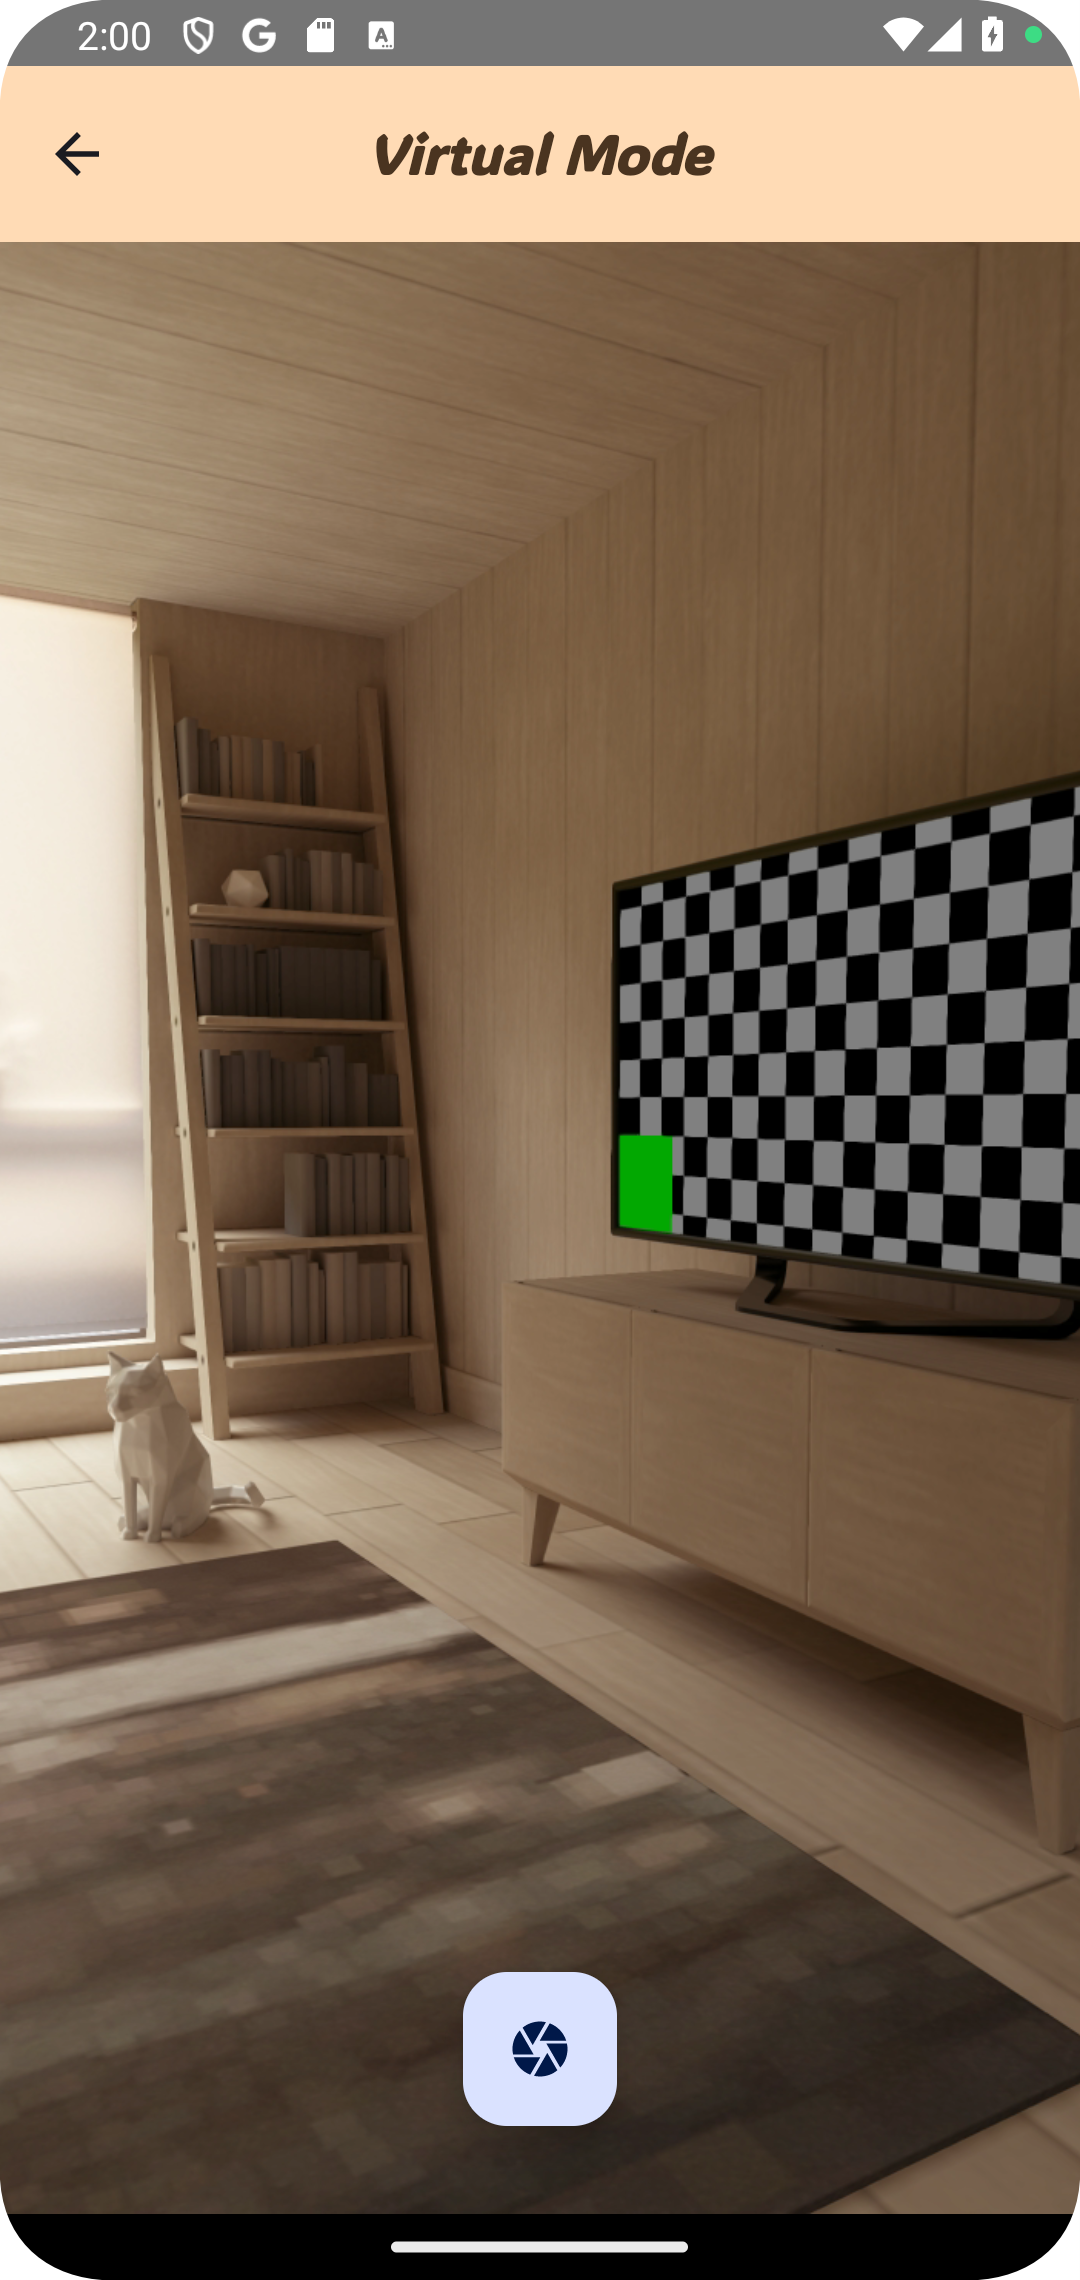
\includegraphics[width=\textwidth]{img/virtual mode.png}
        \caption{Virtual Mode}
        \label{fig:virtual_mode}
    \end{subfigure}
    \hfill
    \begin{subfigure}[b]{0.27\textwidth}
        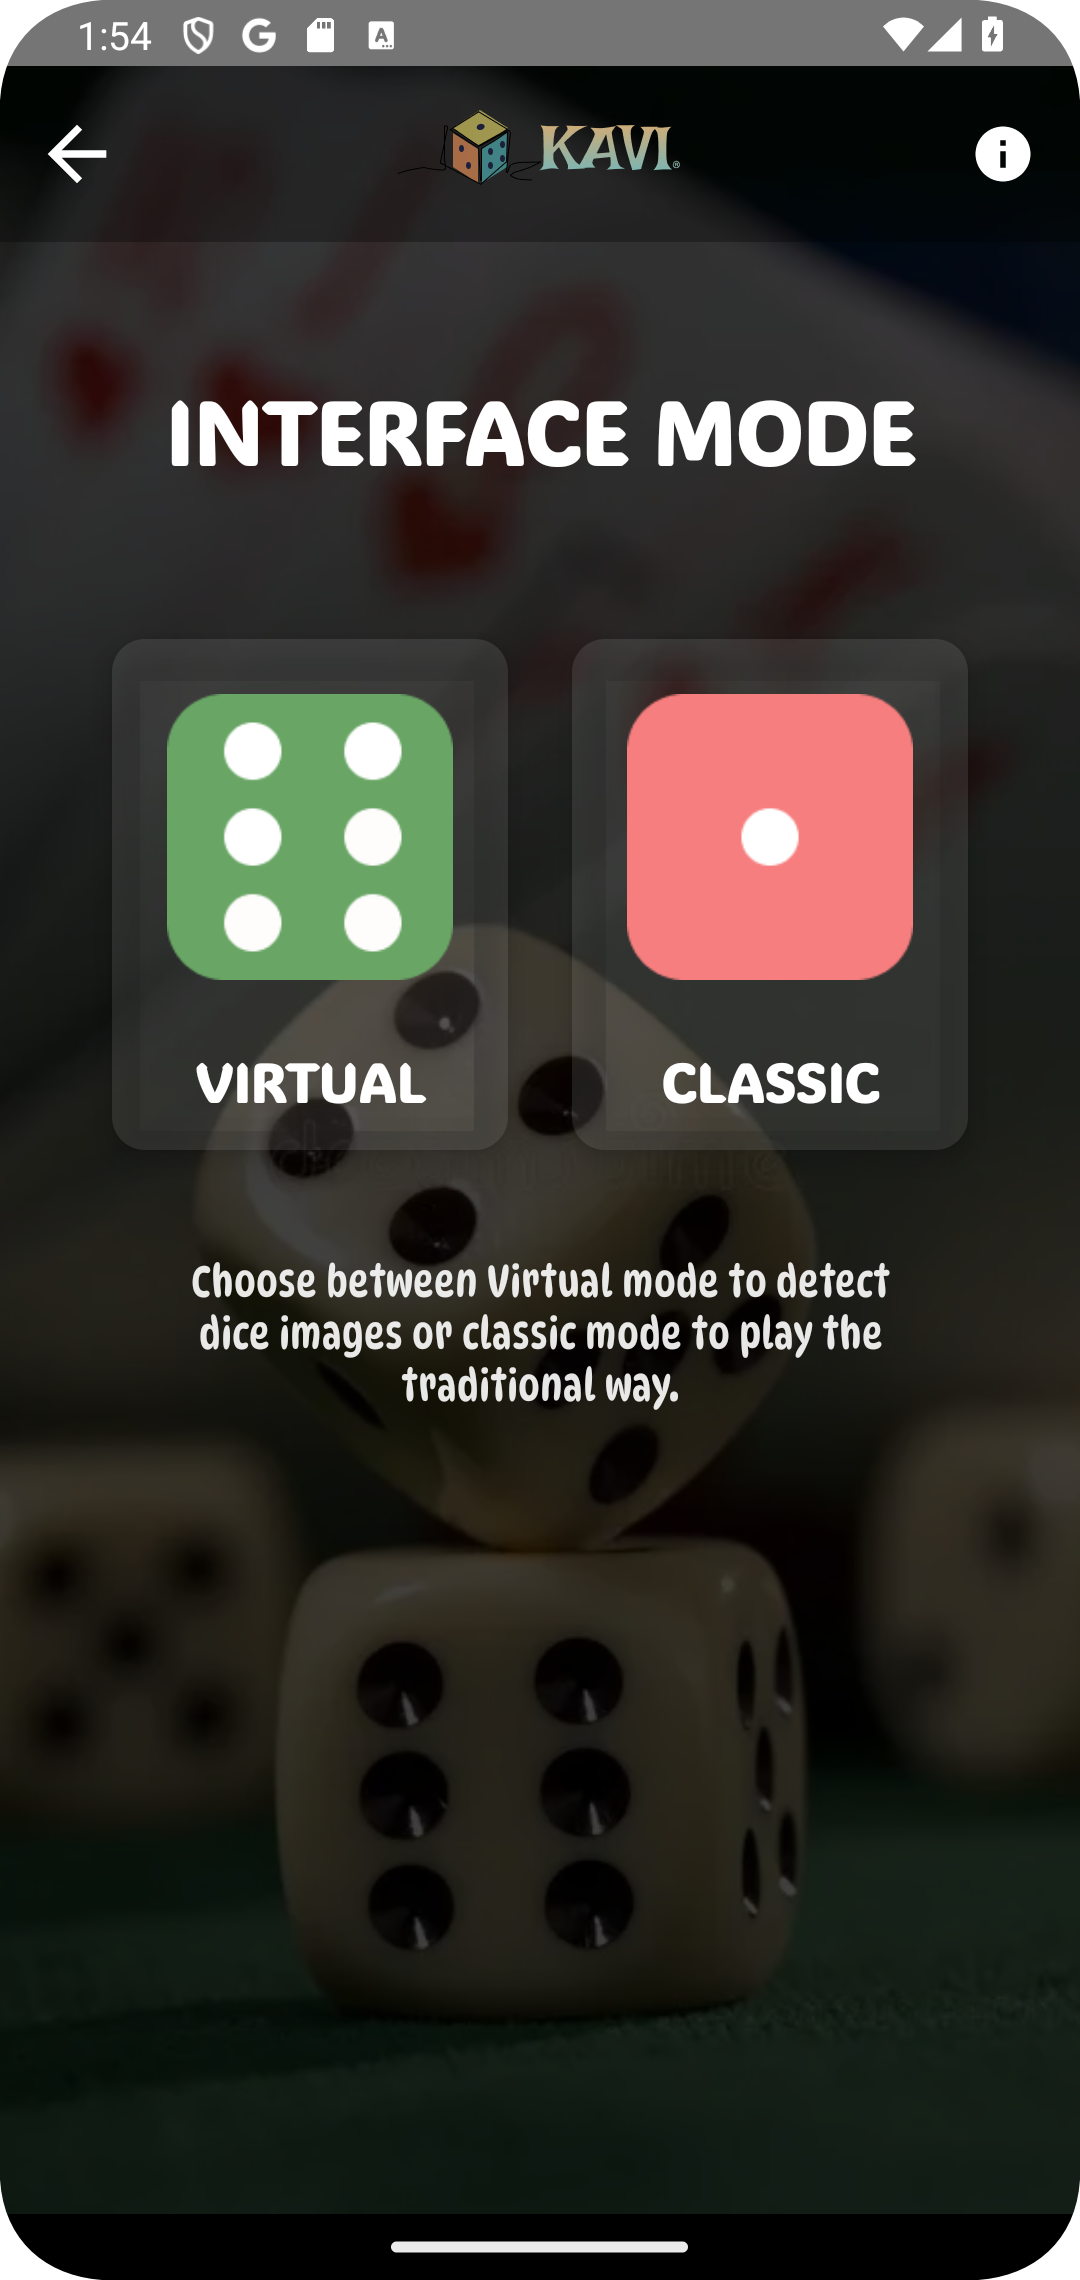
\includegraphics[width=\textwidth]{img/interface mode.png}
        \caption{The Start Screen}
        \label{fig:start_screen}
    \end{subfigure}
    \hfill
    \begin{subfigure}[b]{0.27\textwidth}
        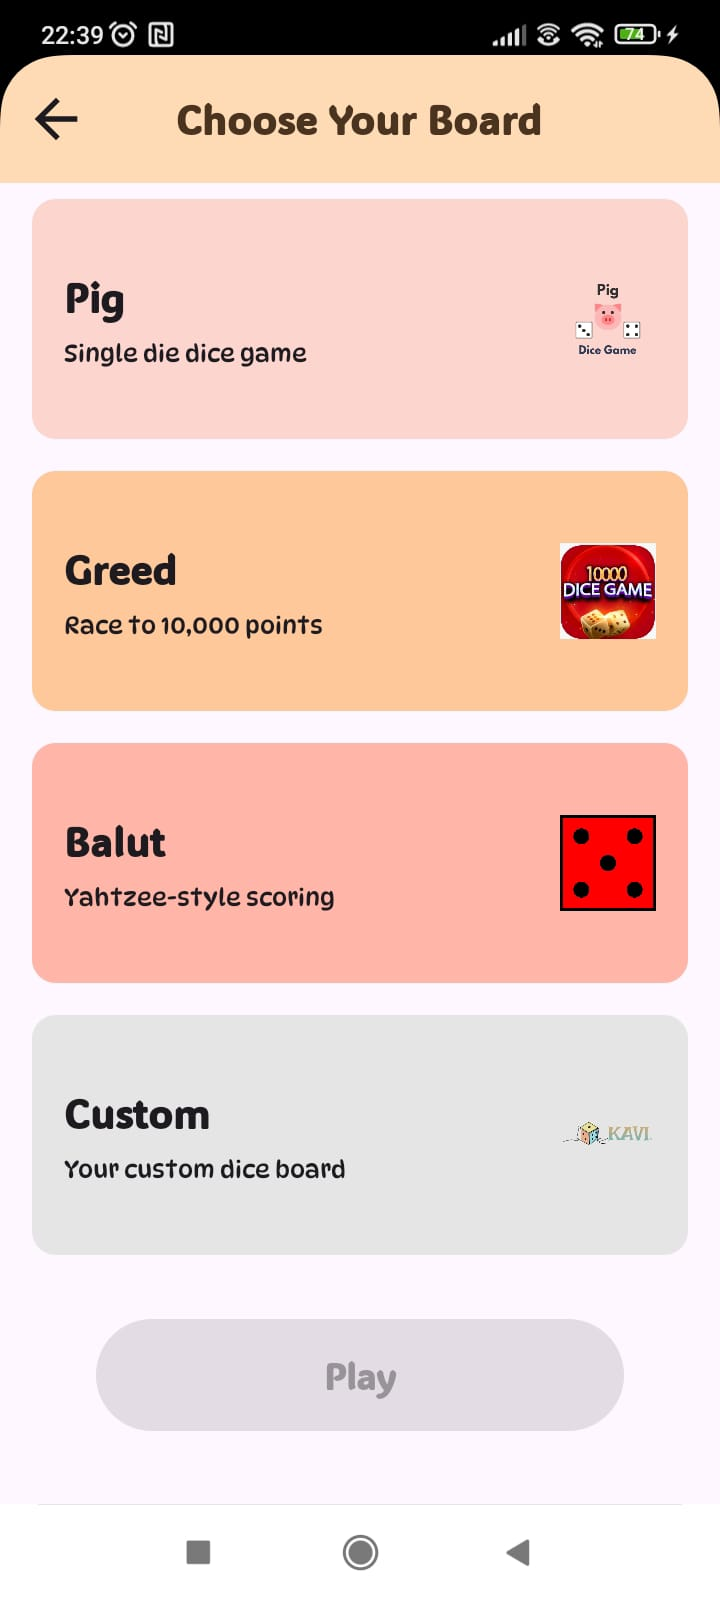
\includegraphics[width=\textwidth]{img/classic boards.jpg}
        \caption{Classic Mode}
        \label{fig:board_screen}
    \end{subfigure}
\caption{The Games main interfaces.}
\label{fig:interface_mode}
\end{figure}

\subsection{Virtual Mode}

Virtual Mode integrates real-time dice detection using the device's camera.  This mode allows users to play with physical dice, enhancing the tactile and interactive nature of the game.  To activate Virtual Mode, navigate to the main menu and select the "Virtual" option (Figure~\ref{fig:virtual_mode}).  The application will then request permission to access the camera.

Once granted, the camera feed will be displayed on screen. Users can position their physical dice within the camera's view. Once the capture or retake button is pressed, the application will detect and recognize the values of the dice.  The detected dice values are displayed on-screen, replacing the camera feed.  If the system fails to accurately detect the dice, users can manually correct the detected values using on-screen controls. This ensures accurate scorekeeping even in challenging lighting or dice configurations.

\subsection{Classic Boards}

The application offers a diverse set of game boards, each designed for a distinct dice game experience. These games range from simple "press-your-luck" scenarios to more strategic challenges that require planning and risk management. The primary games offered are \emph{Pig}, \emph{Greed}, and \emph{Balut}. Additionally, the application includes a custom board where users can define their own game rules and scoring mechanisms, and also select the number of dice used in the game.  Figure~\ref{fig:board_screen} shows the classic boards available in the application.  These games feature an adaptive AI opponent that adjusts its strategy based on the player's performance and the specific game rules.  For a detailed explanation of the AI's behavior in each game, see Section~\ref{subsec:adaptive_ai}.

\begin{figure}[ht!]
    \centering
    \begin{subfigure}[b]{0.27\textwidth}
        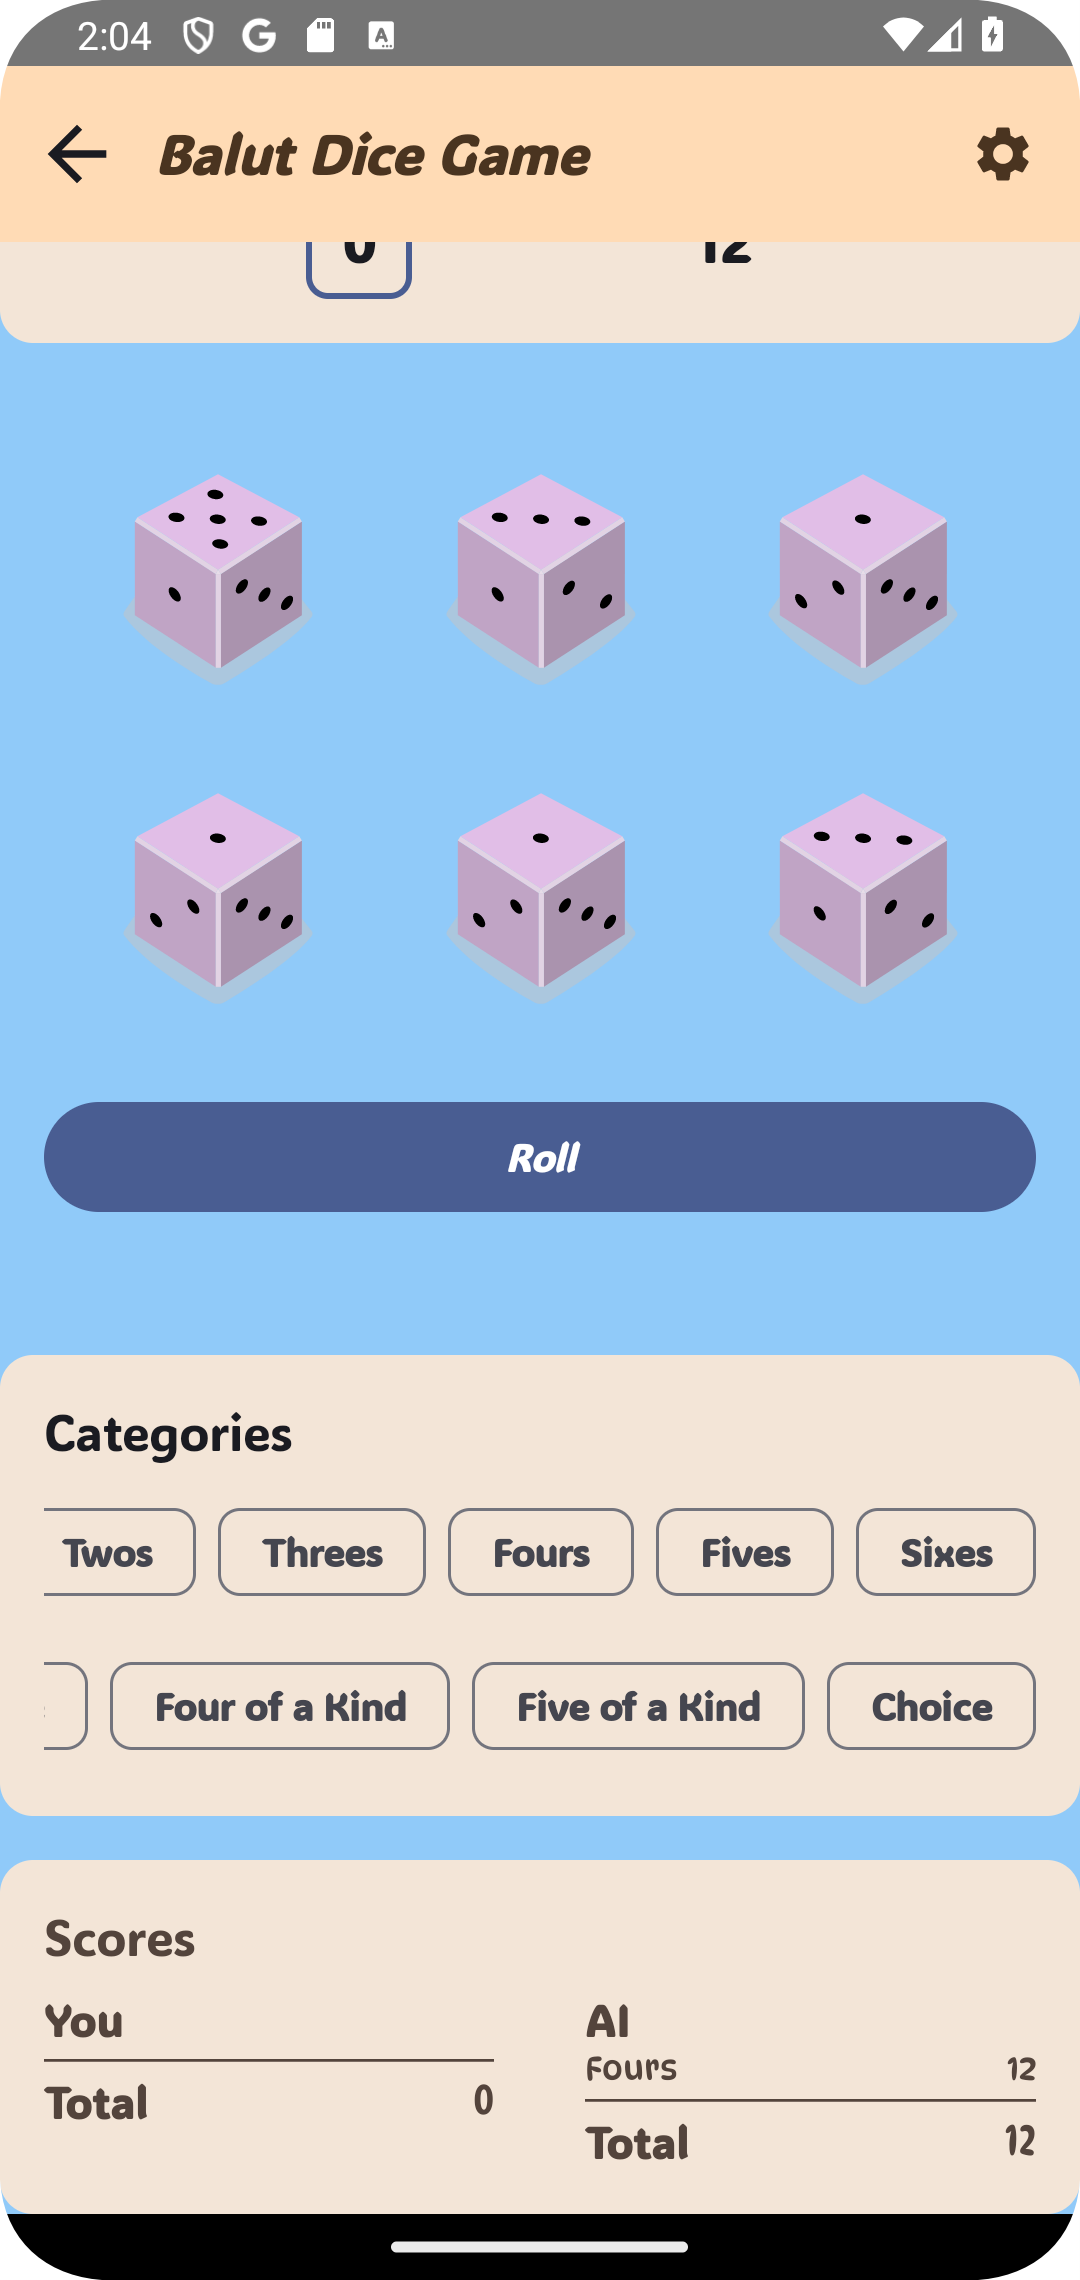
\includegraphics[width=\textwidth]{img/balut board.png}
        \caption{Balut Game Board}
    \end{subfigure}
    \hfill
    \begin{subfigure}[b]{0.27\textwidth}
        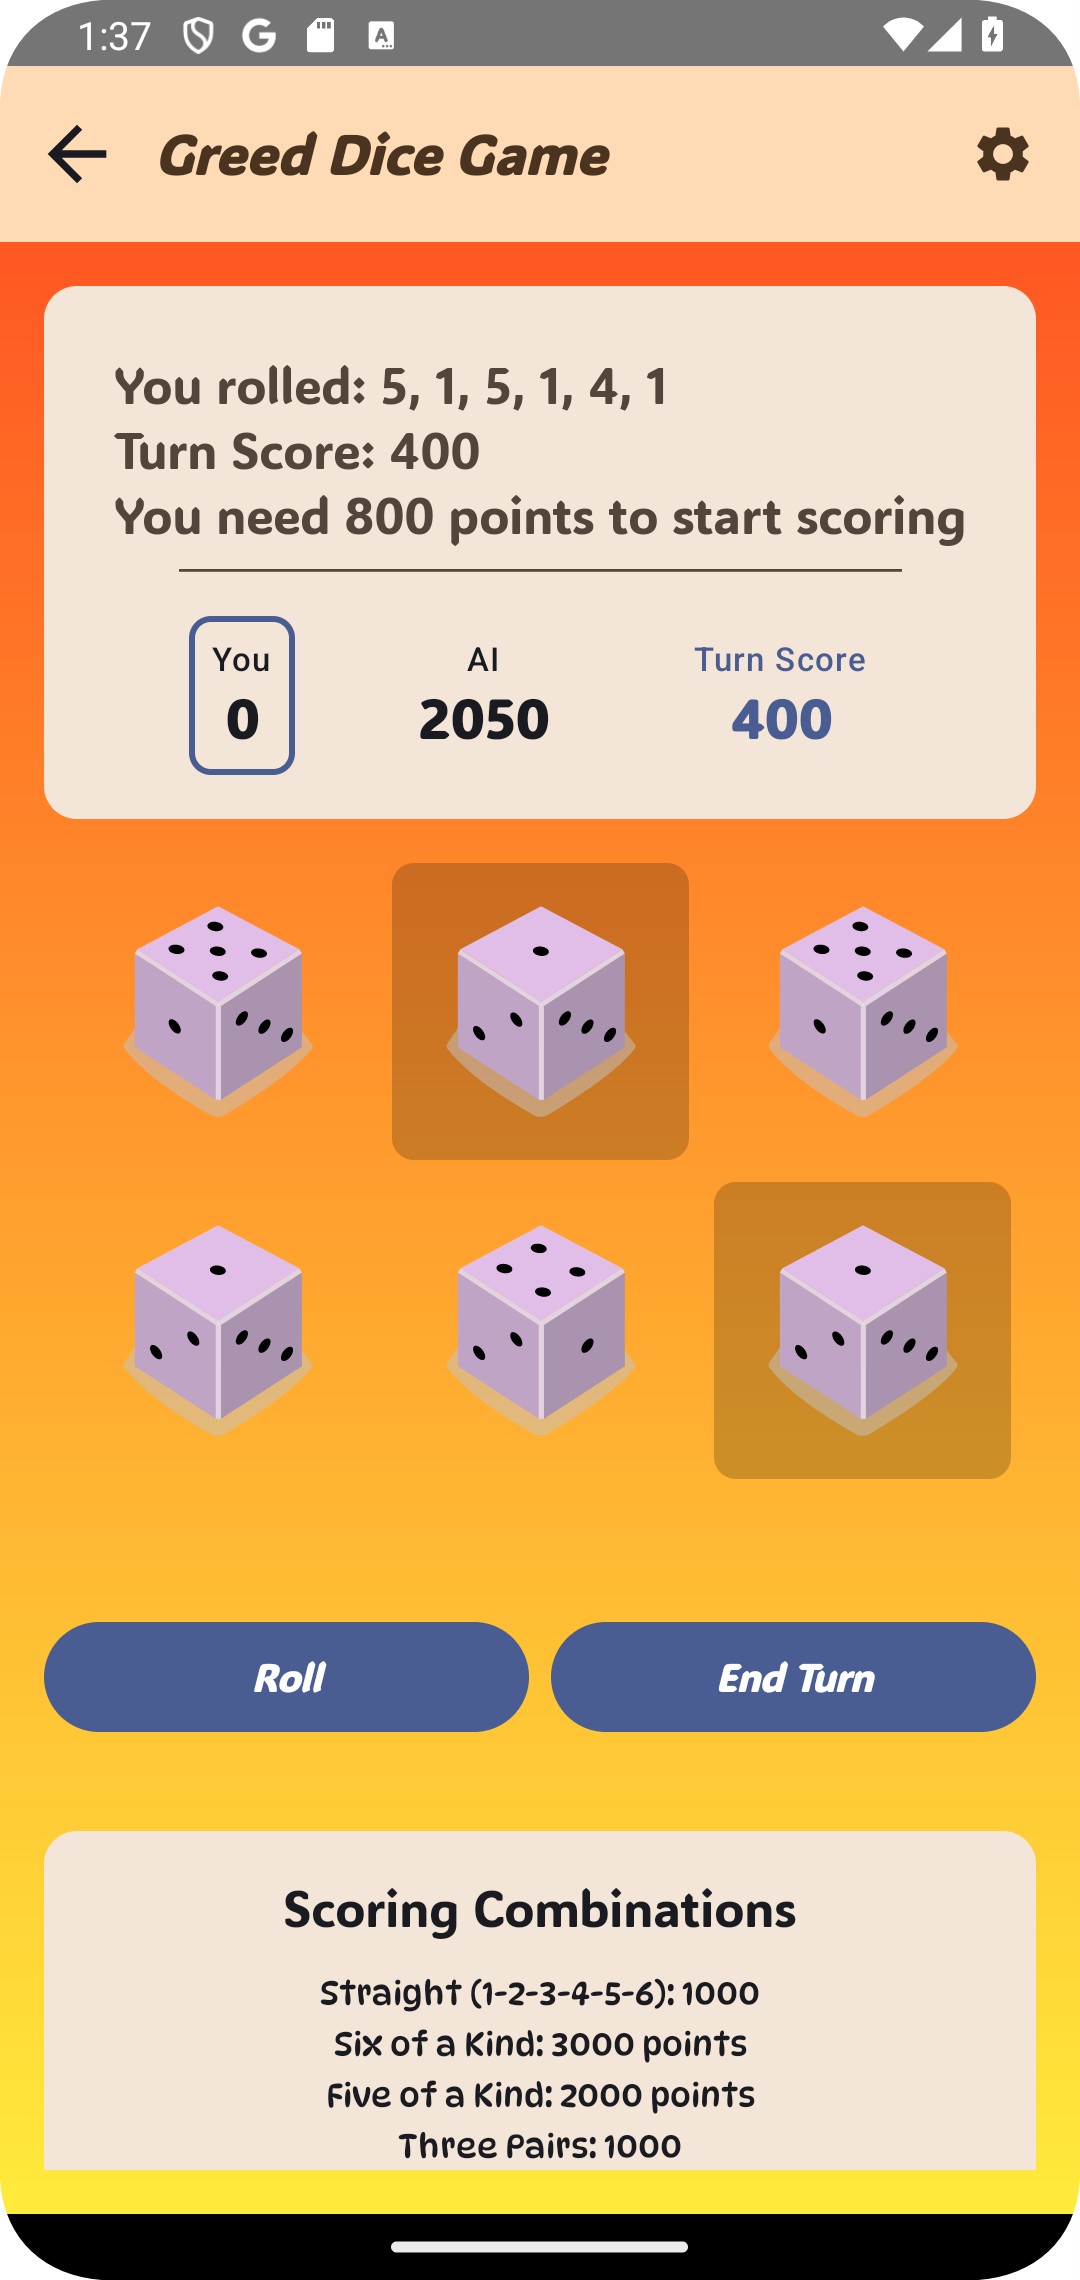
\includegraphics[width=\textwidth]{img/greed board.png}
        \caption{Greed Game Board}
    \end{subfigure}
    \hfill
    \begin{subfigure}[b]{0.27\textwidth}
        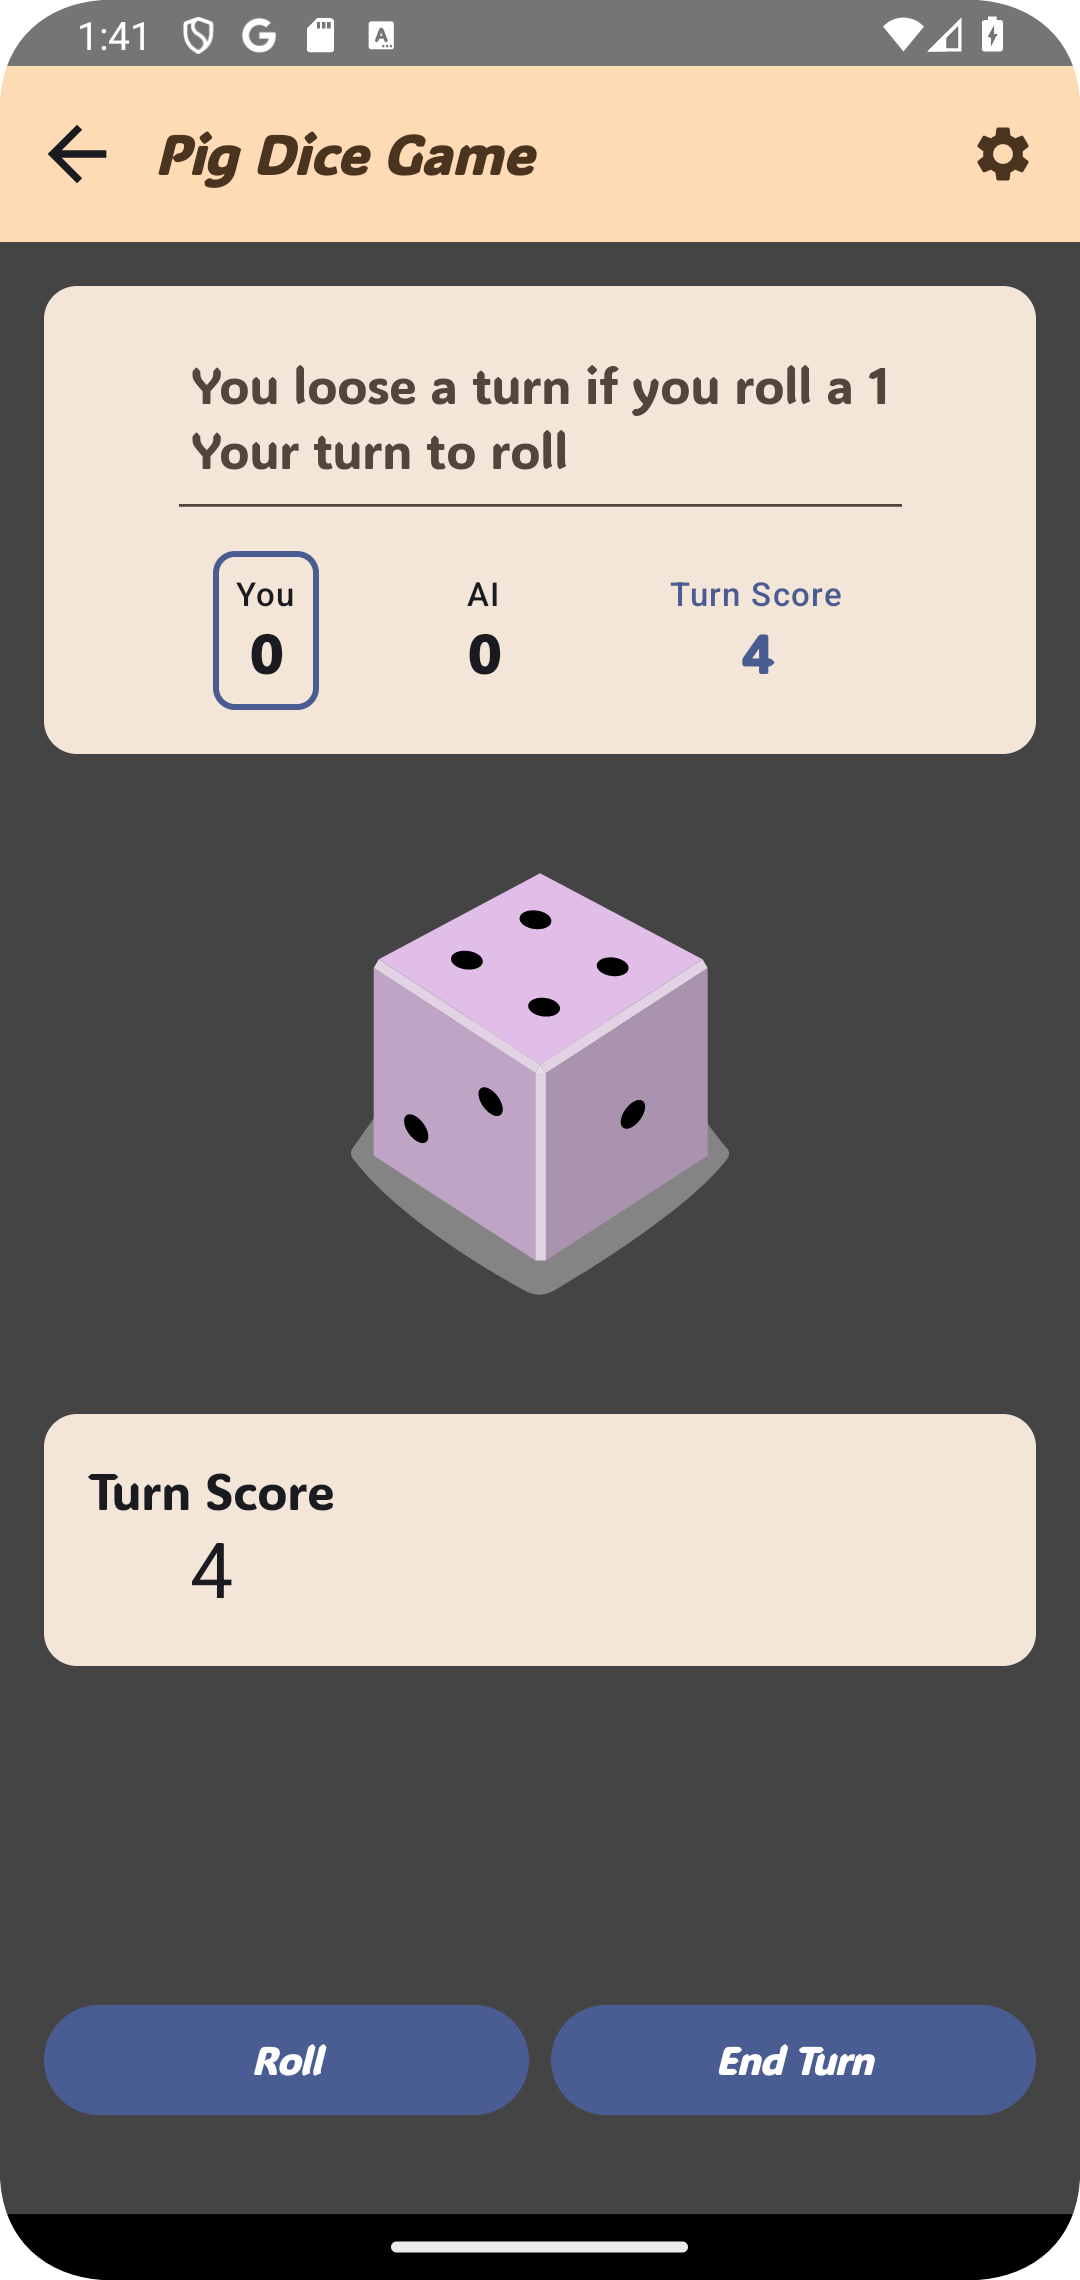
\includegraphics[width=\textwidth]{img/pig board.png}
        \caption{Pig Game Board}
    \end{subfigure}
    \caption{Game Boards in the Application}
    \label{fig:game_boards}
\end{figure}

\subsection{Game Objectives}

\subsubsection{Pig: The Risk of the Roll}

Pig is a simple, engaging game of chance and risk. The goal is to be the first player to reach a total of 100 points. During each turn, players roll a single die, accumulating points with each roll. The key aspect of Pig is the ability to "bank" the points you have accumulated in that turn, however, the risk is that if you roll a 1, you lose all the points accumulated during that turn. The challenge lies in choosing when to press your luck for more points and when to play it safe to avoid losing those points.

\subsubsection{Greed: Navigating Scoring Combinations}

Greed is a more complex game that rewards strategic decision-making and risk-taking. Each turn begins with the roll of six dice. After the roll, players get to select which dice they want to keep to accumulate points, based on scoring combinations like straights, sets (e.g., three-of-a-kind, four-of-a-kind), and single 1s and 5s. These combinations vary in their scoring values, meaning that a key aspect of the game is knowing which combinations you should aim for. Unlike Pig, in Greed, players must accumulate at least 800 points in a turn to start banking them. The winner is the first player to reach a total of 10,000 points.

\subsubsection{Balut: Strategic Category Management}

Balut is a game of strategy, similar to Yahtzee. Players have up to three rolls per turn using five dice. The core of Balut is strategically filling the scoring categories, such as sets, straights, full houses, and more. Each category can be used only once, so planning and smart selection of which dice to hold is critical. After all categories are filled, the player with the highest total score wins. The game boards are shown in Figure~\ref{fig:game_boards}.

\subsection{Game Controls: Interacting with the Game}

The application provides a user-friendly interface with intuitive controls, allowing players to easily interact with each game and manage their scores. This section talks about the various controls and how they function across different game modes.

\subsubsection{Basic Game Controls (Roll, End Turn)}

The primary way players interact with the games is through the roll button. In games like \textit{Pig} and \textit{Greed}, this button (shown in Figure~\ref{fig:control1}) also serves as an "End Turn" button. In these games, tapping the button rolls the dice and also ends the turn after a score is obtained.

\begin{figure}[ht!]
    \centering
    
\includegraphics[width=0.6\textwidth]{img/control1.jpg}
    \caption{Roll and End Turn Button}
    \label{fig:control1}
\end{figure}

\subsubsection{Player Management and Custom Game Setup}

In the custom game board, it is also possible to add players and edit their names (as shown in Figure~\ref{fig:control2}). This function can be accessed by tapping a button which allows the player to add and remove player, as well as edit their names. This allows users to set up a new game of their liking.

\begin{figure}[ht!]
    \centering
    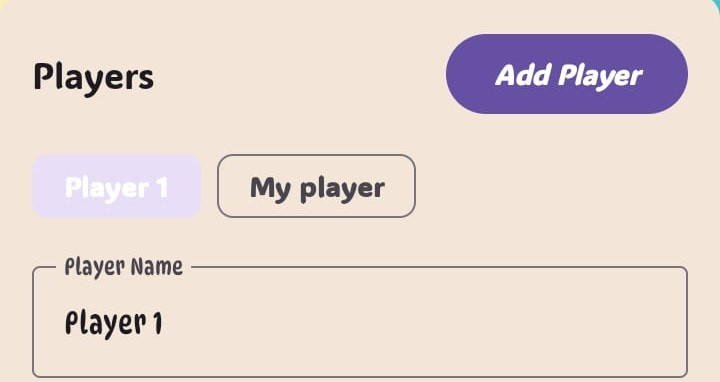
\includegraphics[width=0.6\textwidth]{img/control2.jpg}
    \caption{Player Management and Editing}
    \label{fig:control2}
\end{figure}

\subsubsection{Balut-Specific Controls (Category Selection)}

\textit{Balut} introduces the unique feature of category selection. After rolling the dice, a player can select a category in which to score, shown in Figure~\ref{fig:control3}. This allows for a more strategic game, where each category can only be used once.

\begin{figure}[ht!]
    \centering
    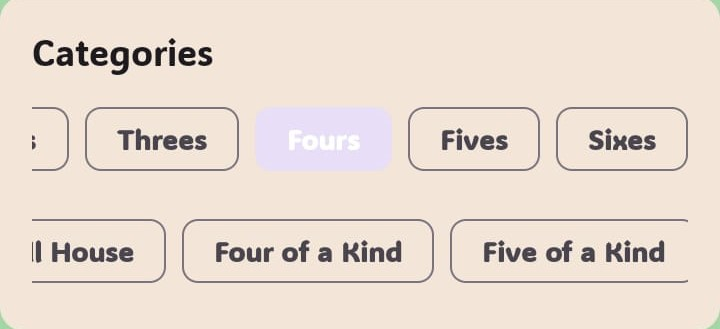
\includegraphics[width=0.6\textwidth]{img/control3.jpg}
    \caption{Balut Category Selection}
    \label{fig:control3}
\end{figure}

\subsubsection{Holding Dice}

In both \textit{Greed} and \textit{Balut}, players can strategically select dice to hold for the next roll. As seen in Figure~\ref{fig:control4}, this is done by tapping on the individual dice on the screen. The selected dice will be saved, and can be rolled again in the subsequent roll.

\begin{figure}[ht!]
    \centering
    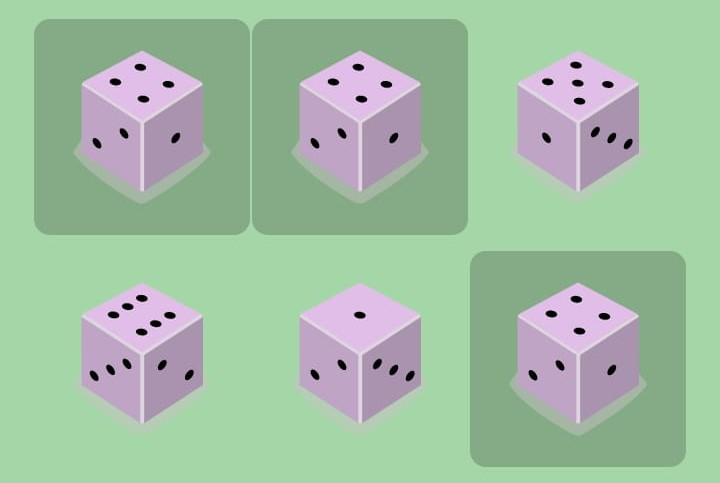
\includegraphics[width=0.6\textwidth]{img/control4.jpg}
    \caption{Selecting Dice to Hold}
     \label{fig:control4}
\end{figure}

\subsubsection{Balut Score Function}

After a category has been selected in \textit{Balut}, the game also provides an additional button which can be tapped to calculate the score and end the turn. As seen in Figure~\ref{fig:control5}.

\begin{figure}[ht!]
    \centering
    
\includegraphics[width=0.6\textwidth]{img/control5.jpg}
    \caption{Balut Roll and Score Button}
    \label{fig:control5}
\end{figure}

\subsubsection{Custom Board Settings}

The custom board allows players to set the number of dice that will be used for that specific game. In addition, the board name can also be set, as seen in Figure~\ref{fig:control6}. This level of customization gives the users control over how the games are played.

\begin{figure}[ht!]
    \centering
    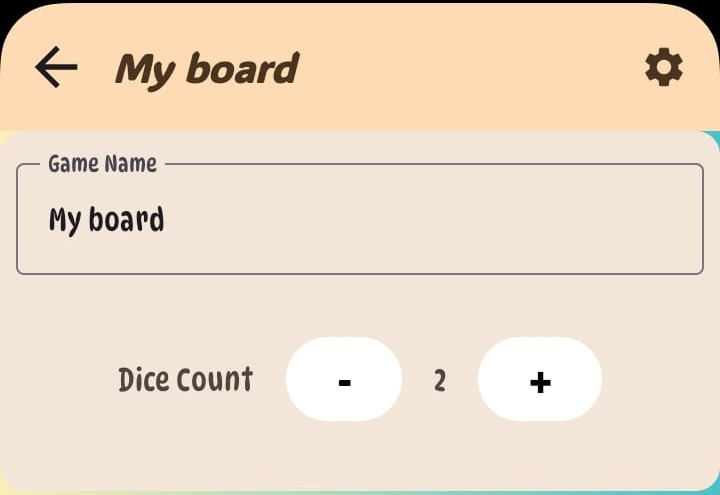
\includegraphics[width=0.6\textwidth]{img/control6.jpg}
    \caption{Custom Board Settings}
    \label{fig:control6}
\end{figure}

\subsubsection{Score Modifiers and Reset}

Figure~\ref{fig:control7} shows the score modifiers, which enable users to manually adjust their scores. This feature can also be used to keep track of score in other types of games that might not be covered by this application, or in the custom mode. The feature also contains a reset score button that will reset the score of the game to 0. This can be used to easily restart any game or any other custom use. Additionally, this interface also contains the functionality of adding a note that will be saved as part of the game, which can be used to keep track of important information of the current game.

\begin{figure}[ht!]
    \centering
    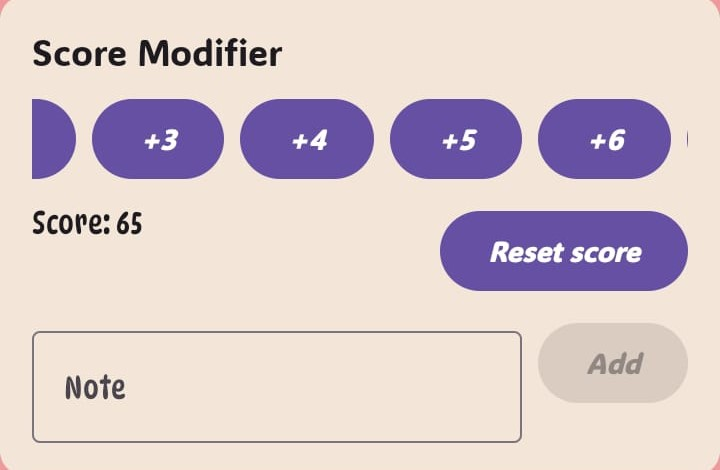
\includegraphics[width=0.6\textwidth]{img/control7.jpg}
    \caption{Score Modifiers and Reset}
     \label{fig:control7}
\end{figure}

\subsection{Instruction}

The instructions screen provides users with detailed guidance on how to play the game. It includes rules, tips, and strategies to enhance the gaming experience. The instructions screen is illustrated in Figure~\ref{fig:instructions_screen}.

\subsection{Settings}
The settings screen, on the other hand, allows users to customize their gaming experience, such as enabling vibration, the shake-to-roll function, and board color customization. The settings screen is shown in Figure~\ref{fig:settings_screen}.

\begin{figure}[ht!]
    \centering
    \begin{subfigure}[b]{0.27\textwidth}
        \centering
        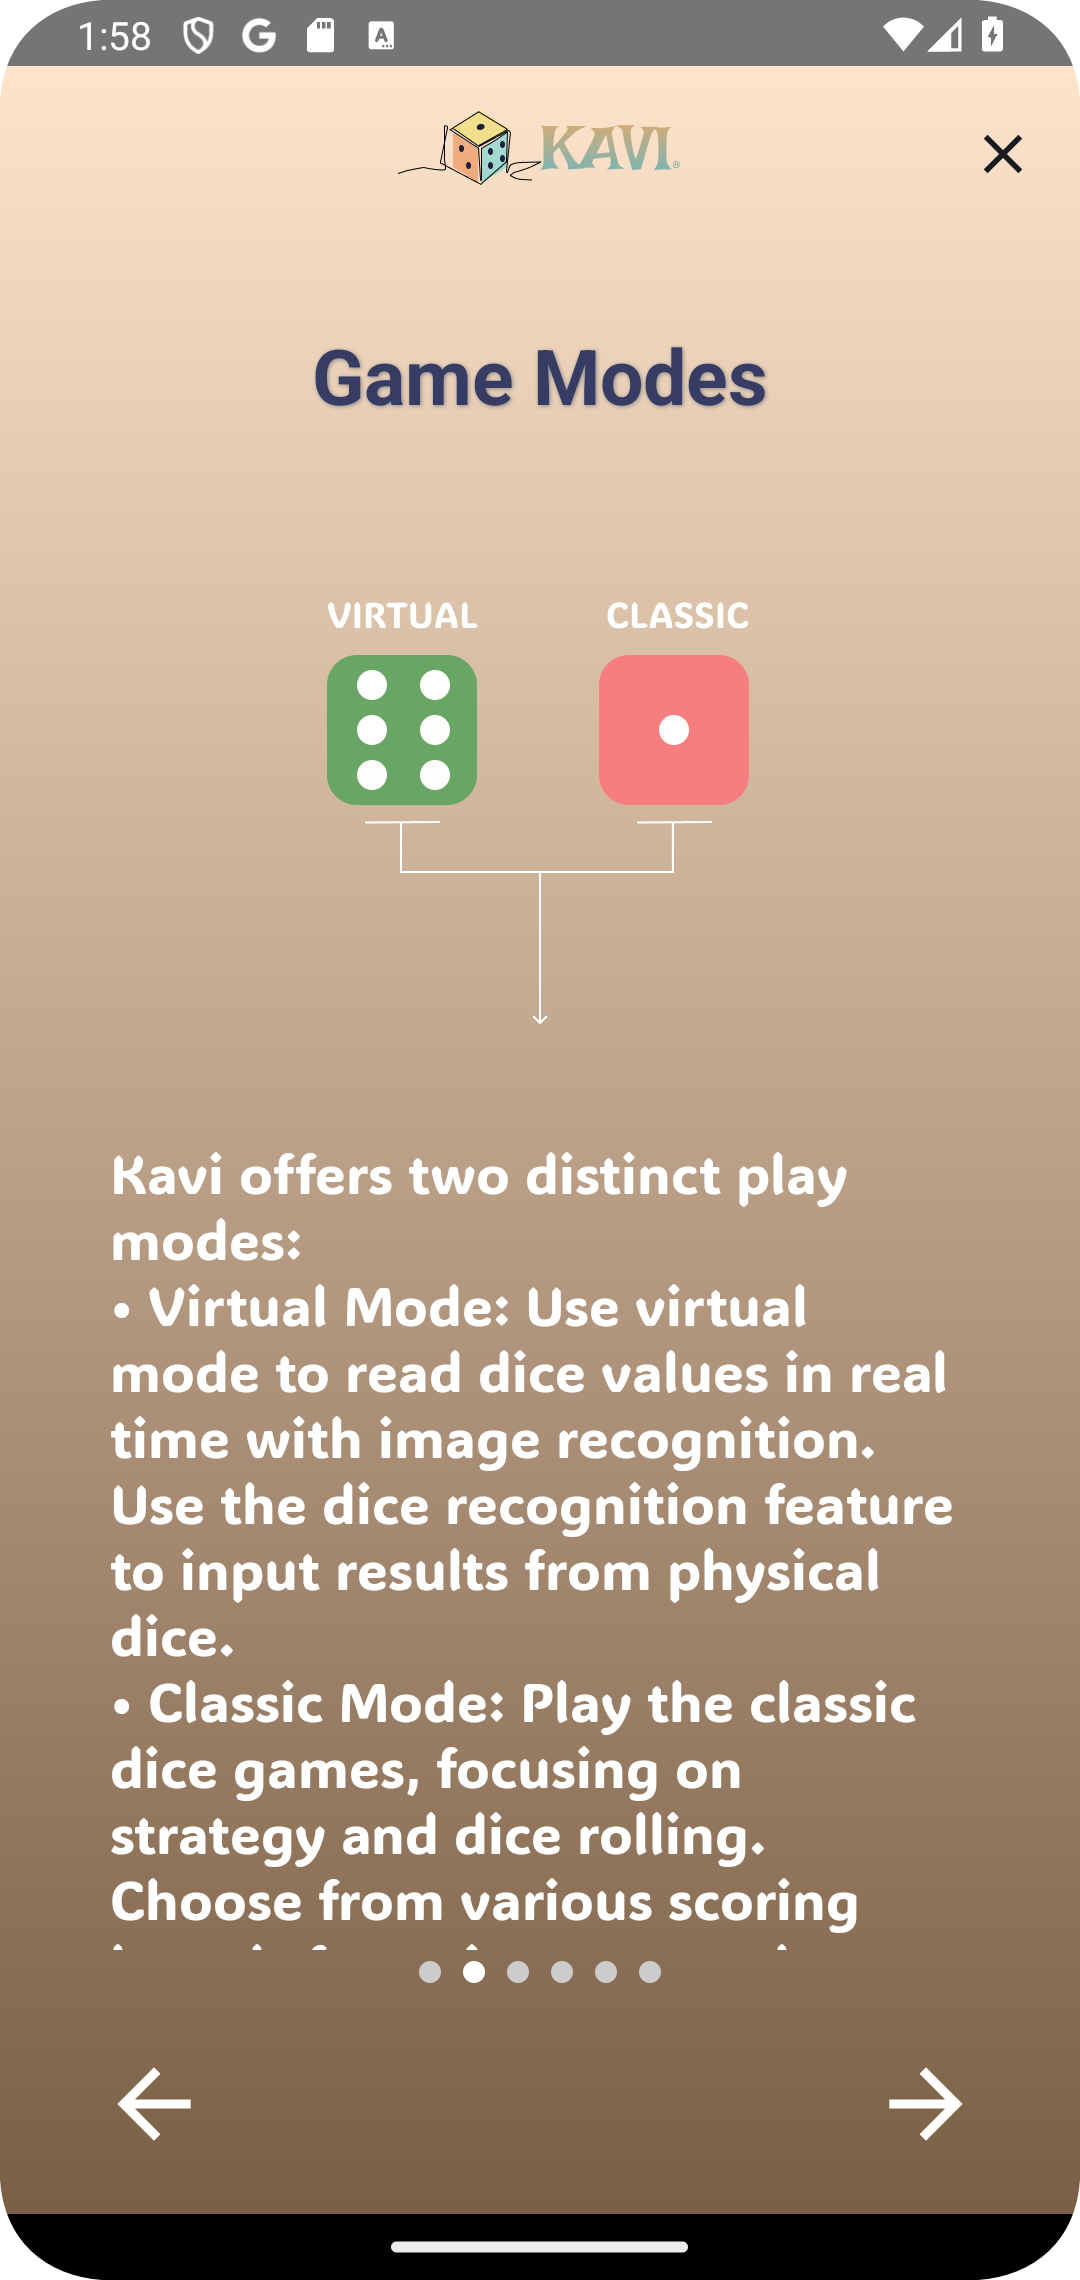
\includegraphics[width=\textwidth]{img/instructions screen.png}
        \caption{Instructions Screen}
        \label{fig:instructions_screen}
    \end{subfigure}
    \hspace{.5em}
    \begin{subfigure}[b]{0.27\textwidth}
        \centering
        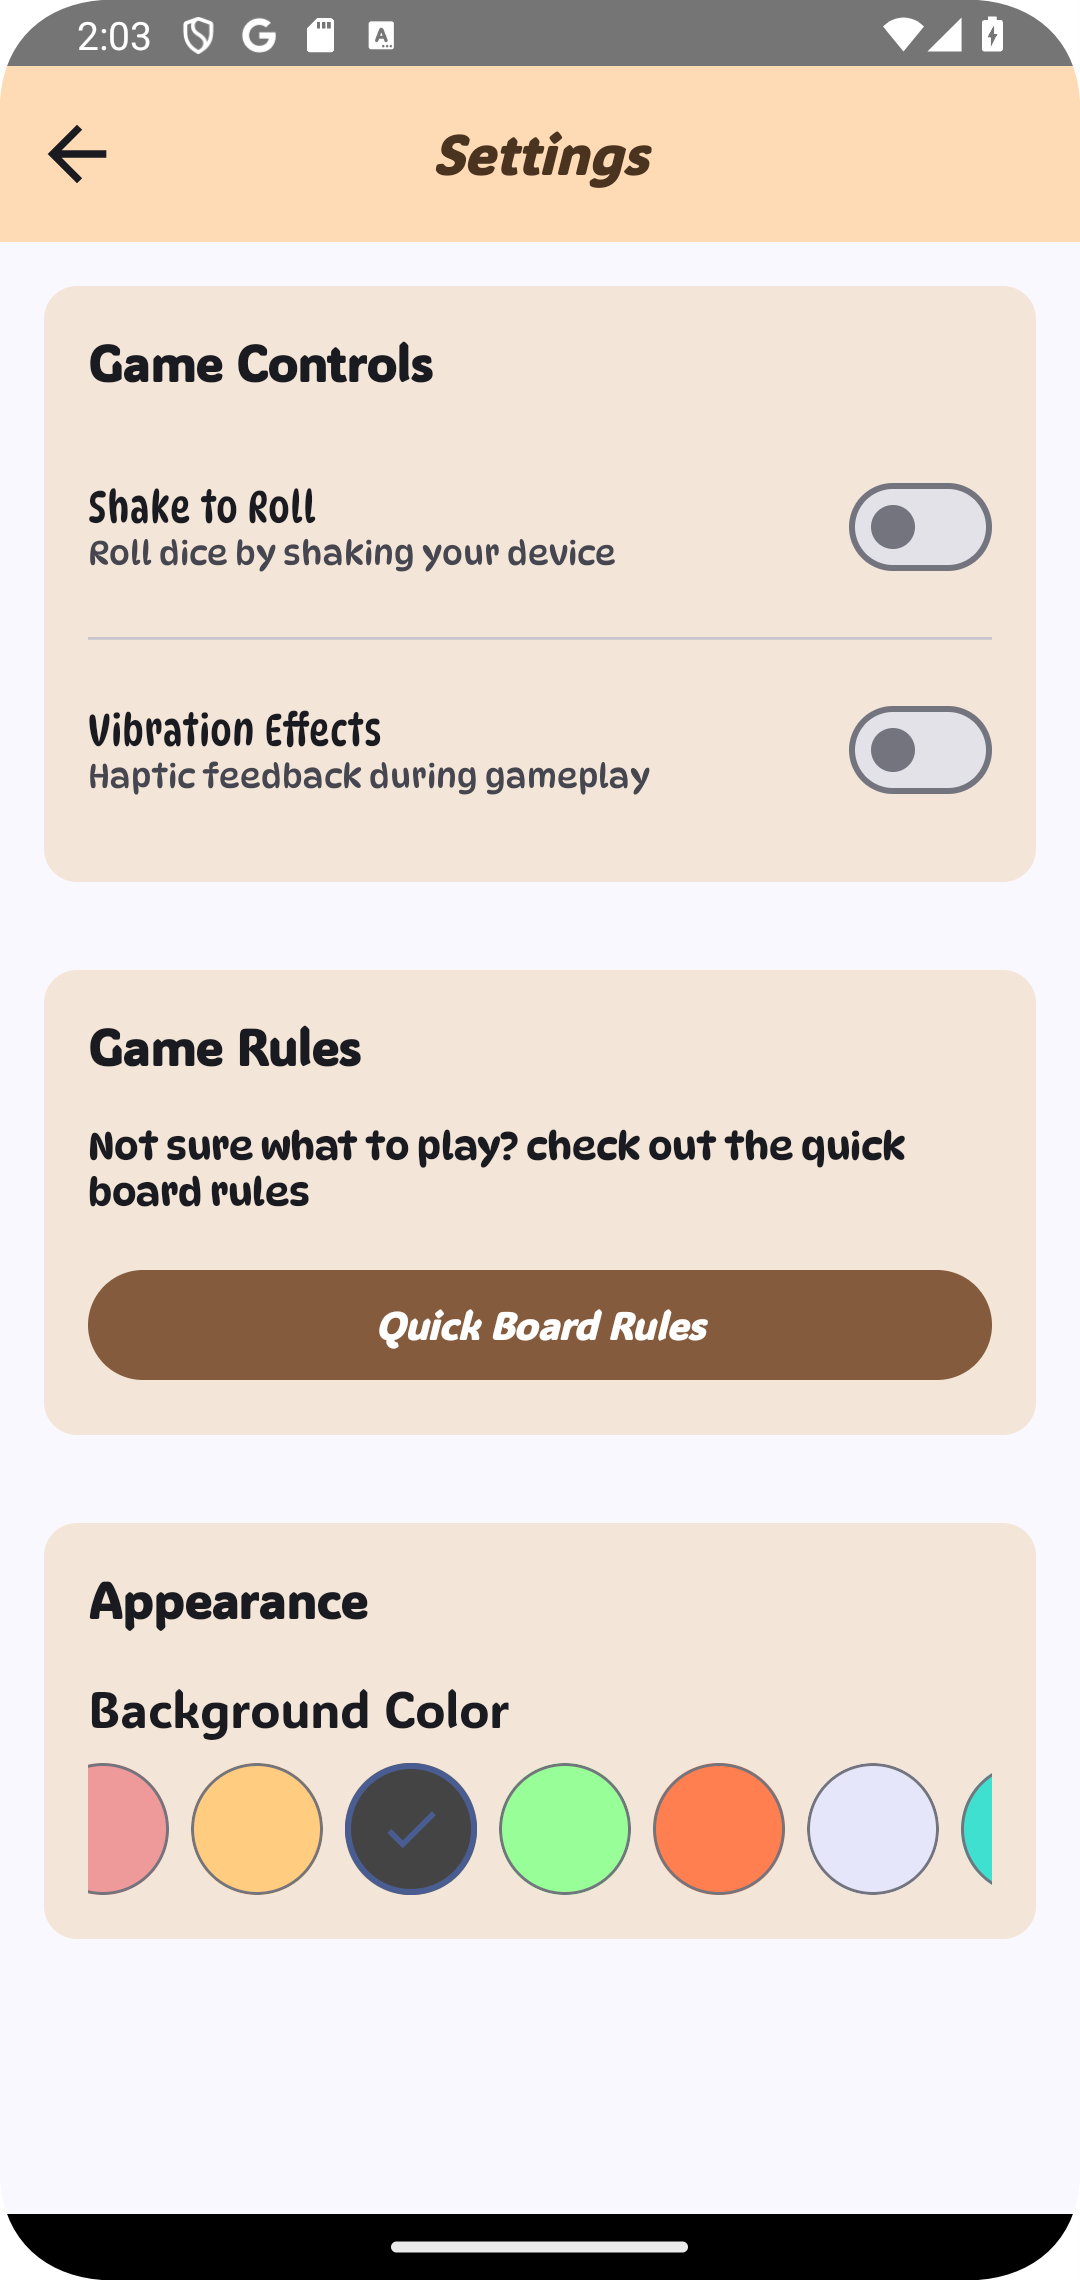
\includegraphics[width=\textwidth]{img/settings screen.png}
        \caption{Settings Screen}
        \label{fig:settings_screen}
    \end{subfigure}
    \caption{Instructions and Settings.}
\end{figure}

\subsection{Statistics}

The statistics screen offers users comprehensive insights into their gameplay performance. It displays a variety of data, including win records, average scores, and other pertinent metrics. The Figure~\ref{fig:statistics_screen} illustrates the statistics screen, where users can view their achievements, such as "High Roller," "Lightning Fast," and "Greed Guru." Additionally, users can assess their risk-taking tendencies, current winning streaks, comebacks, and close games. The screen also features time analytics, allowing users to track their fastest games, total playtime, and time spent on individual games, providing a detailed overview of their gaming habits.
\begin{figure}[ht!]
    \centering
    \begin{subfigure}[b]{0.27\textwidth}
        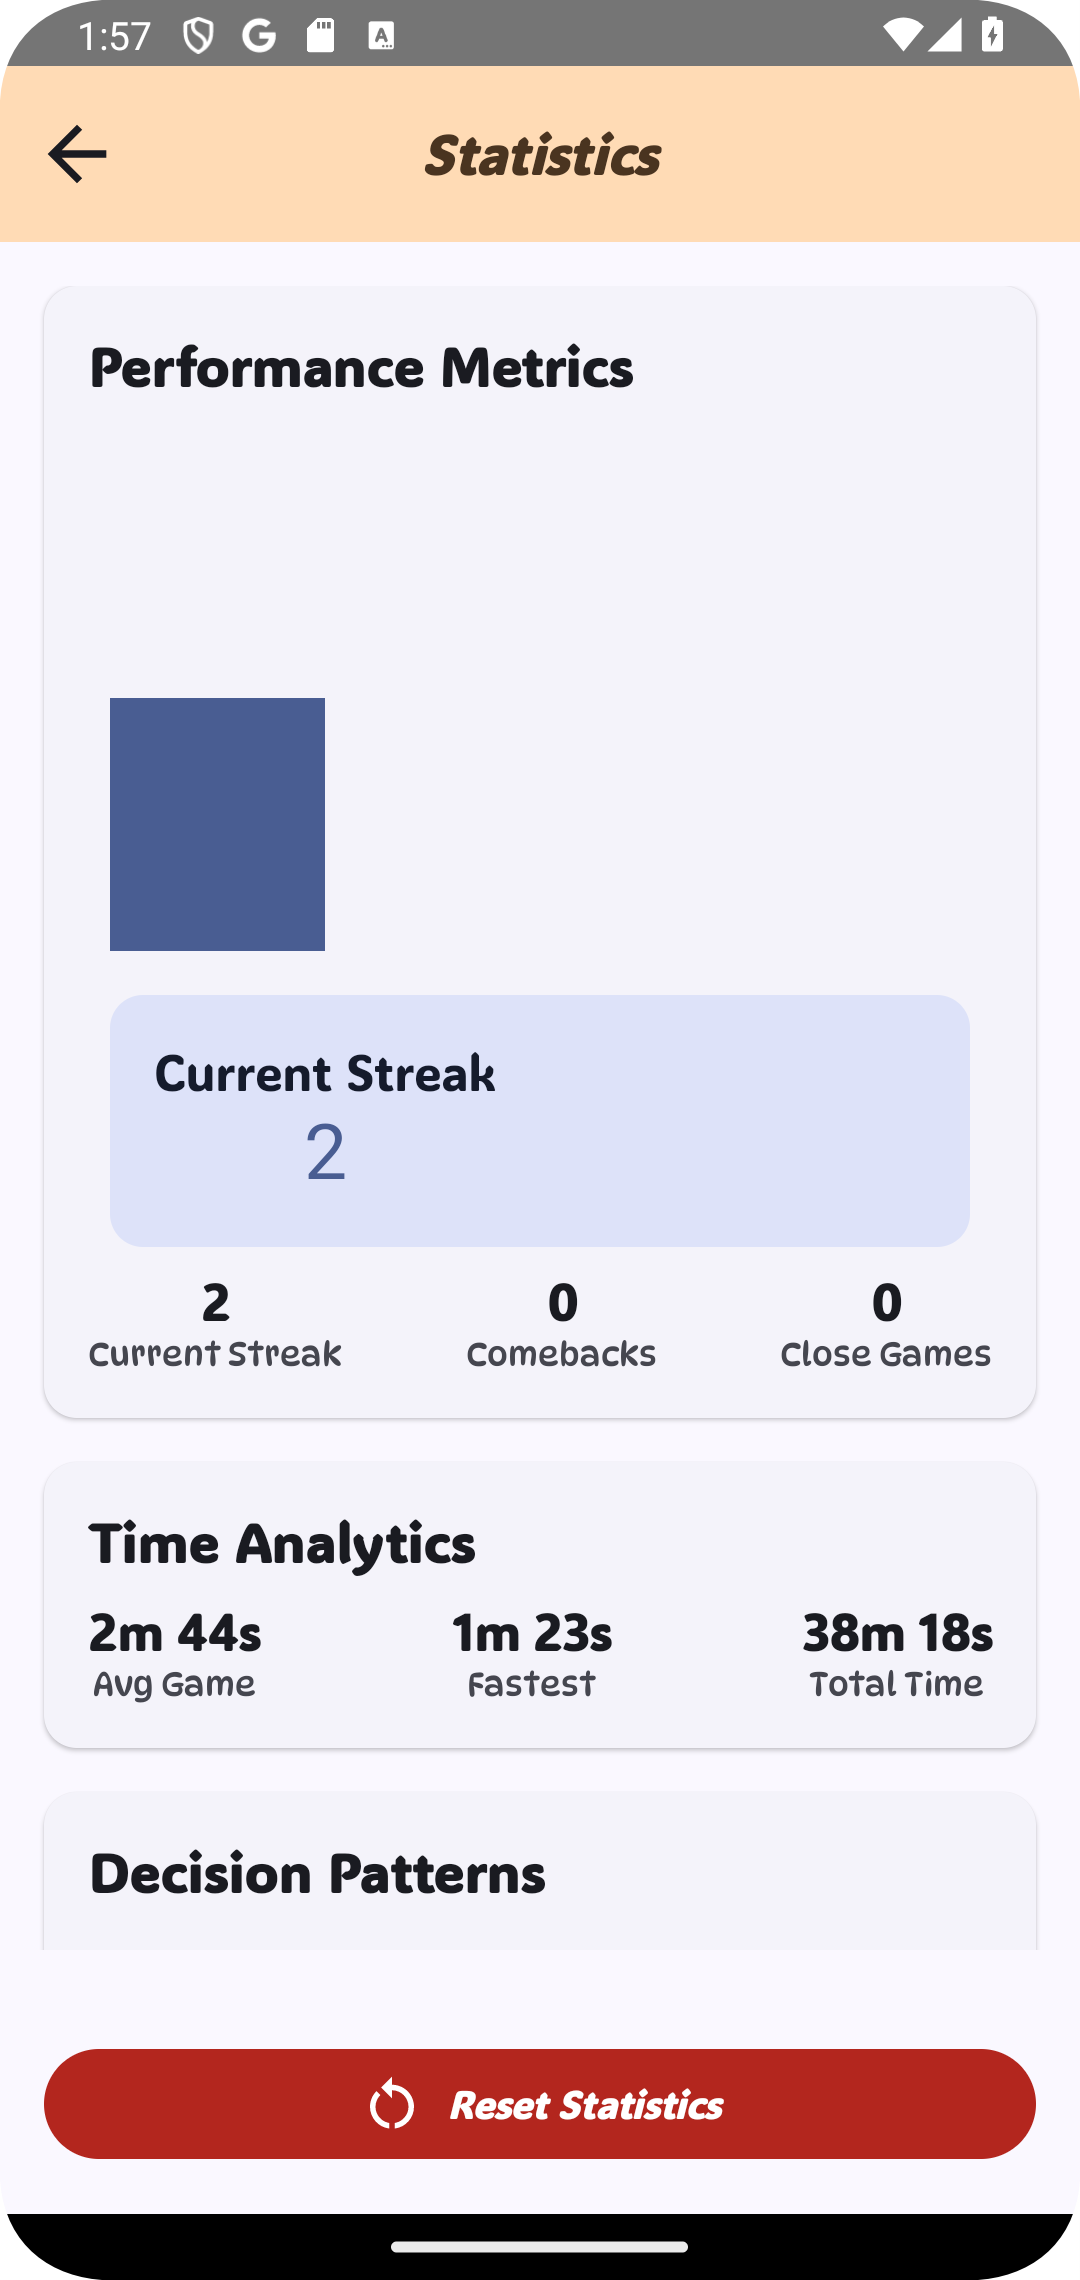
\includegraphics[width=\textwidth]{img/statistics screen.png}
        \caption{Performance Metrics}
    \end{subfigure}
    \hfill
    \begin{subfigure}[b]{0.27\textwidth}
        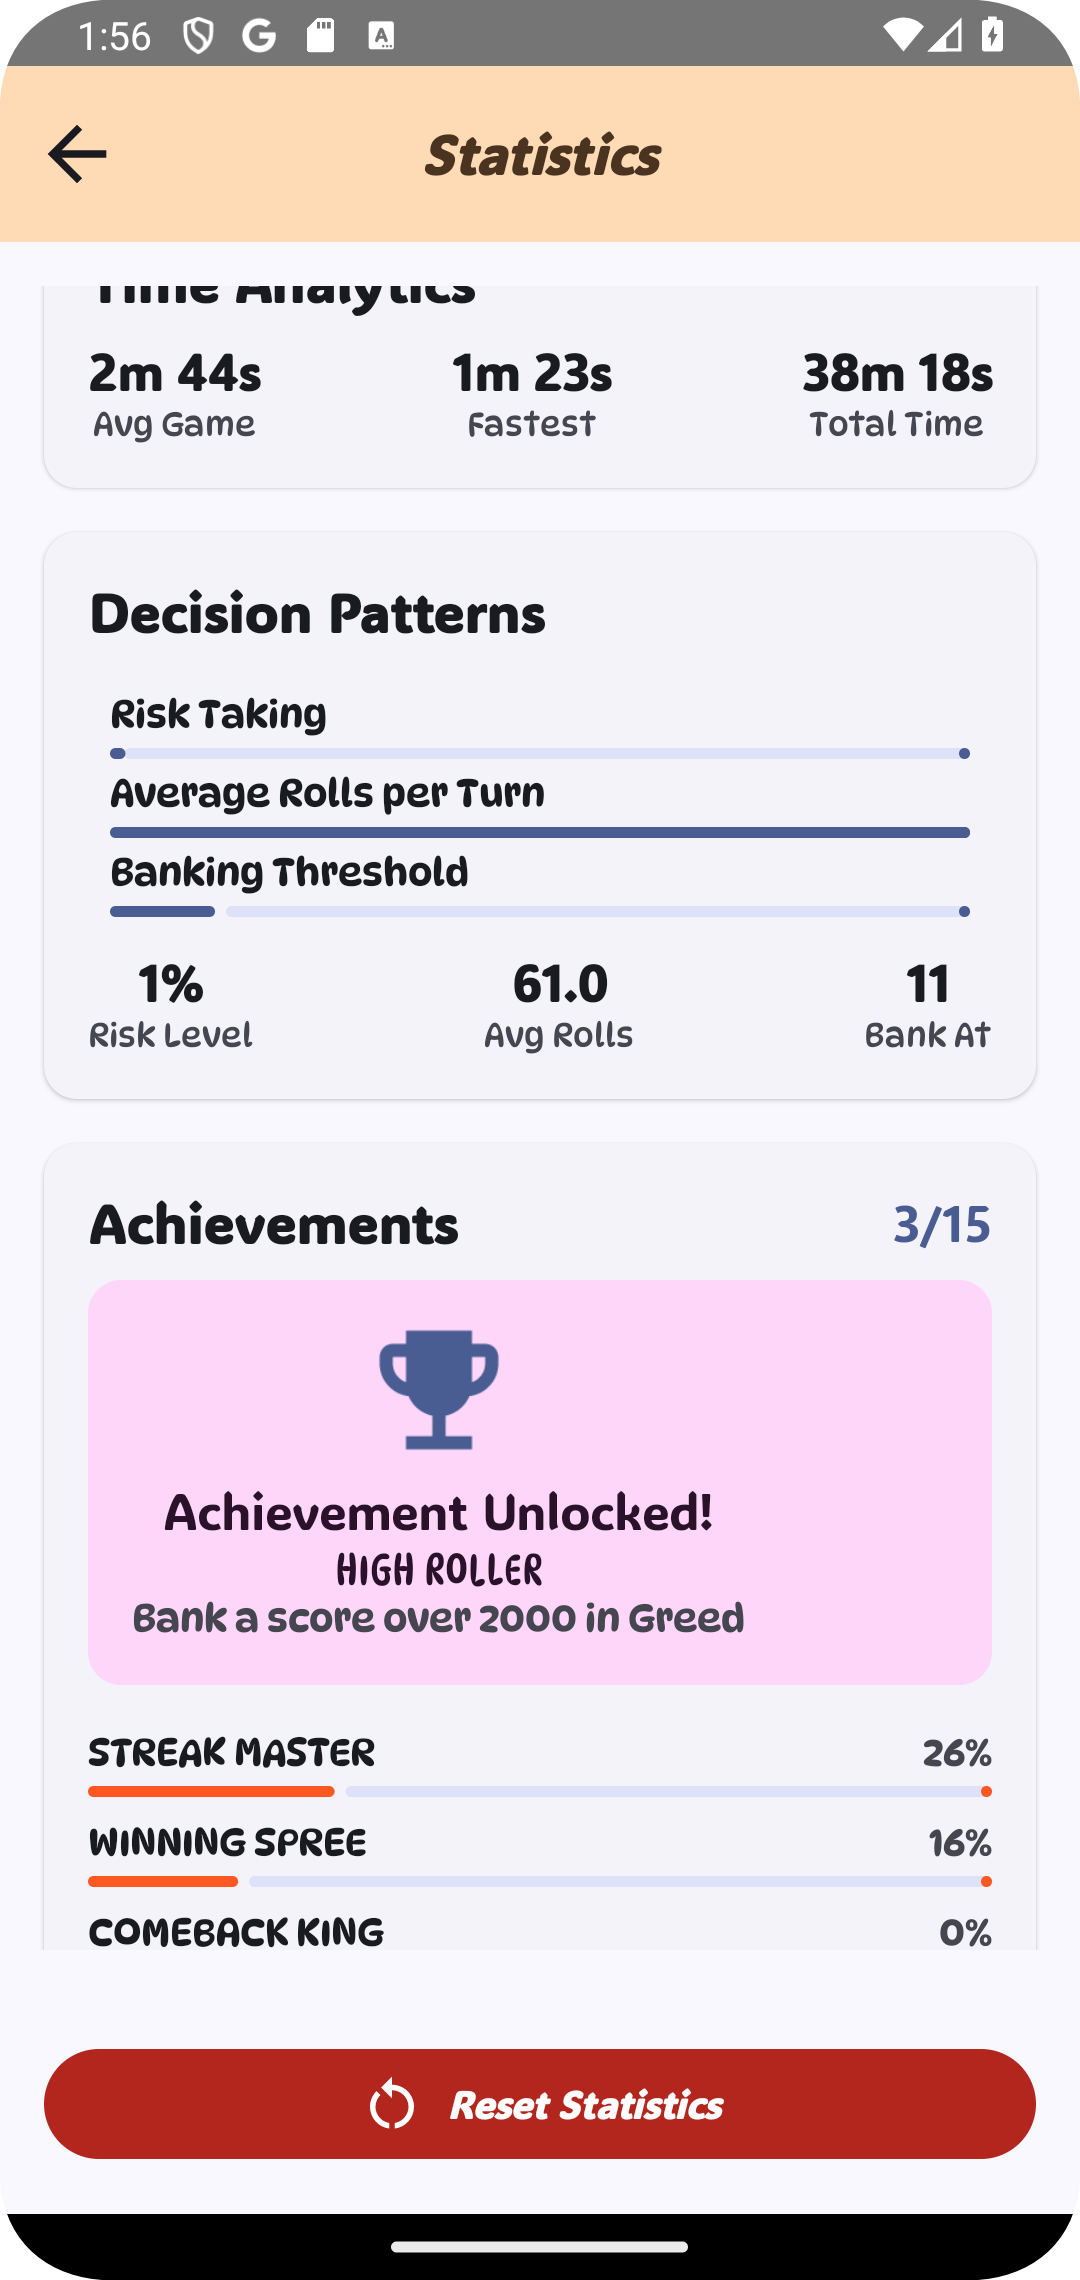
\includegraphics[width=\textwidth]{img/statistics screen3.png}
        \caption{Decision Patterns}
    \end{subfigure}
    \hfill
    \begin{subfigure}[b]{0.27\textwidth}
        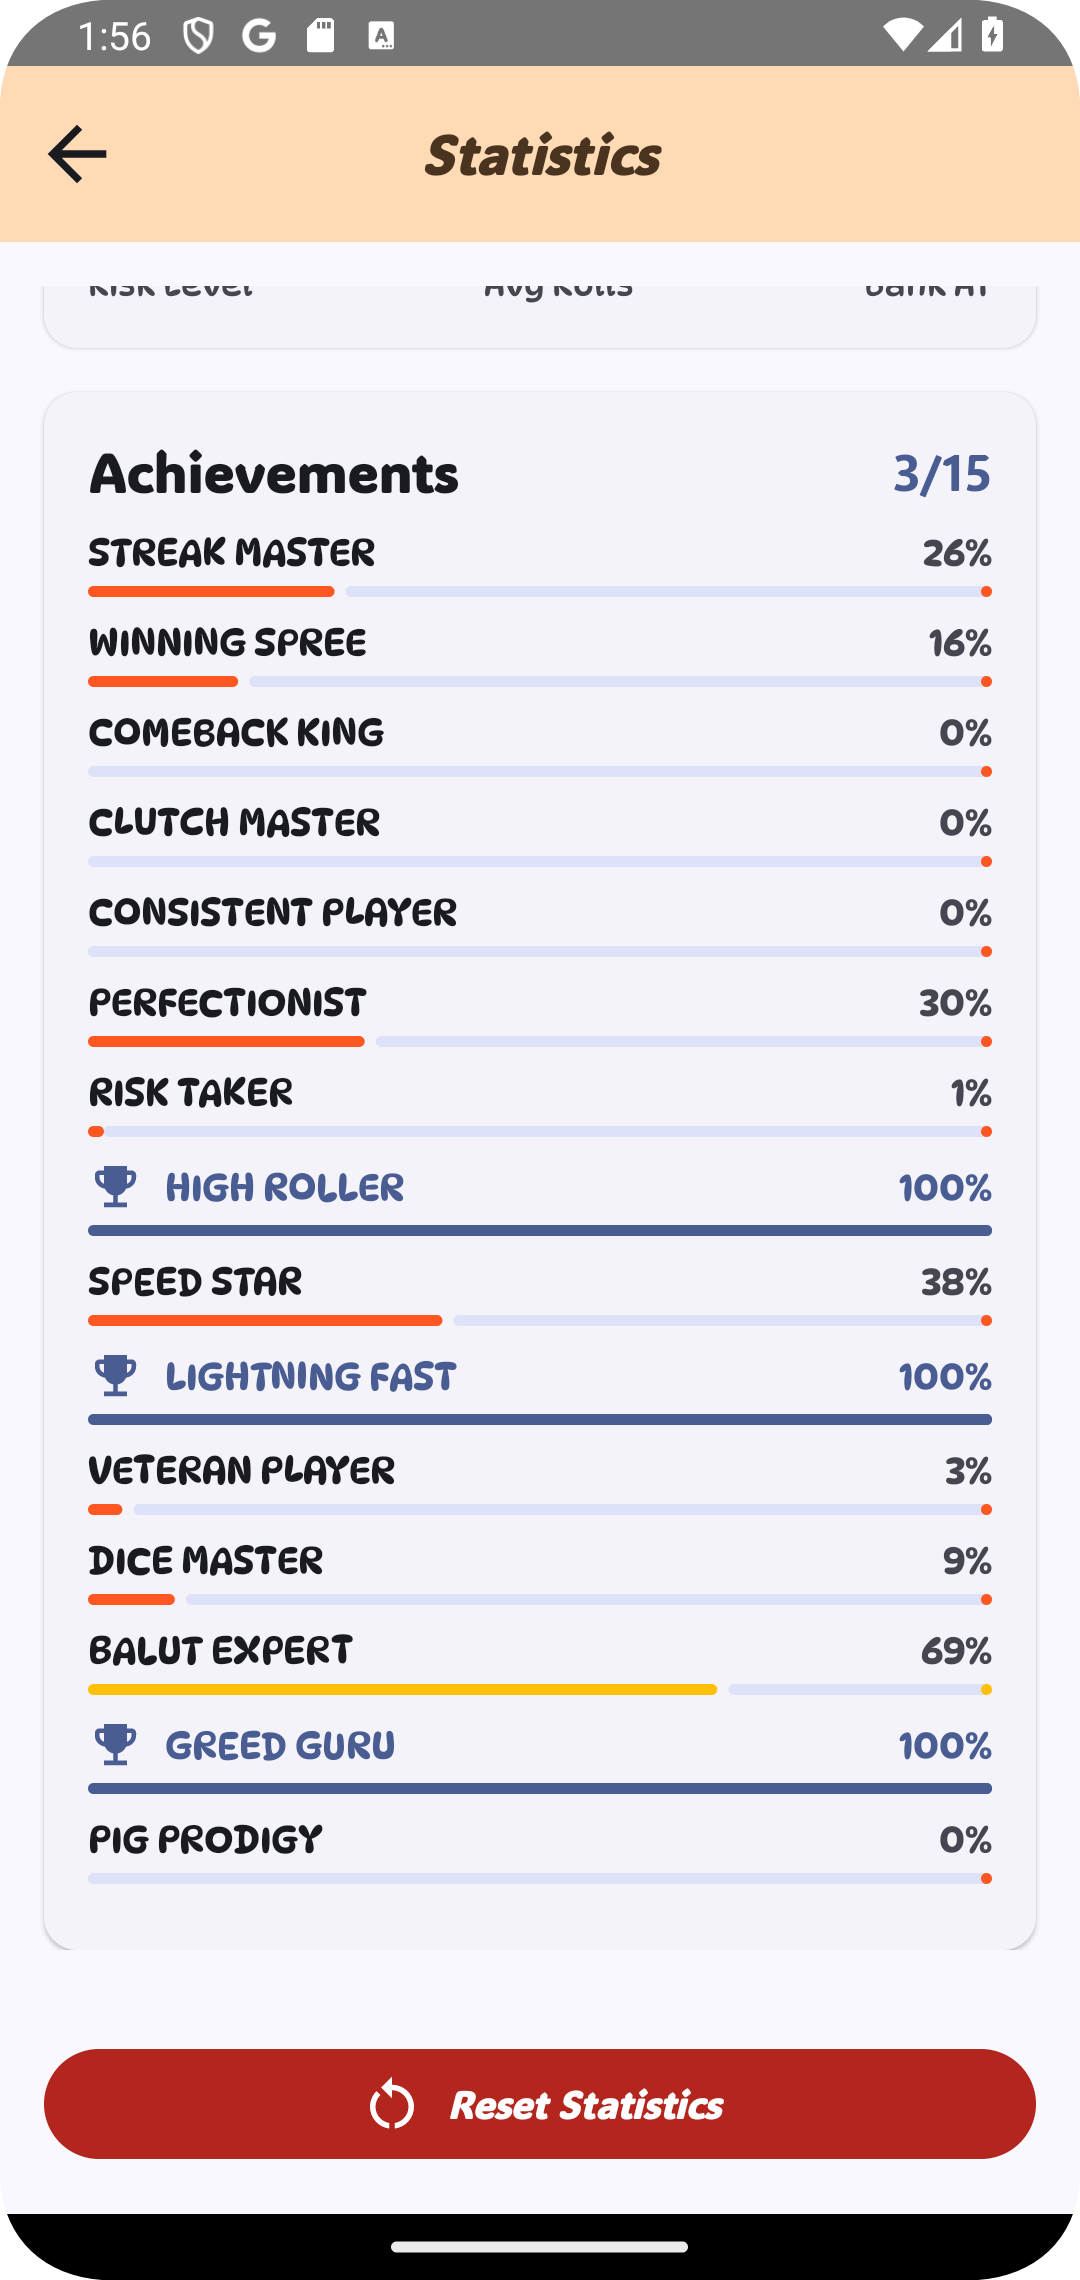
\includegraphics[width=\textwidth]{img/statistics screen2.png}
        \caption{Unlocking Achievements}
    \end{subfigure}
    \caption{Statistics Screen}
    \label{fig:statistics_screen}
\end{figure}

\section{System Administration}

The administration of the application involves several key tasks to ensure its reliability, performance, and security. These responsibilities are primarily carried out by the developers of the application, and can range from day to day maintenance to handling the occasional unforeseen issues.

\subsection{Application Maintenance}

Regular maintenance of the application is essential to ensure it remains functional and up to date. This involves several tasks, including:

\begin{itemize}
    \item \textbf{Release Management:} New releases of the application are periodically deployed via GitHub as APK releases, which often require careful planning and testing to ensure compatibility and maintain a consistent user experience. This includes creating new release branches, building the APK, and updating the app with new changes, new features, or bug fixes.
    \item \textbf{Monitoring and Troubleshooting:} Developers are also responsible for monitoring the performance of the application. This may involve checking for crashes, logging error reports, identifying bugs or unexpected behavior, and making changes to solve the issues.
\end{itemize}

\subsection{Data Management}

Careful management of the application data is critical to ensure its proper functioning.  The developers are responsible for \textit{DataStore Management}, which involves taking periodic backups of application settings and user preferences stored with Android DataStore. The data is also cleaned periodically to ensure that the device is not using unnecessary storage. This is essential to maintain consistency and avoid potential data corruption or data loss.

\section{Security Issues}
This section provides a detailed overview of the various security risks that the application may be vulnerable to, based on potential threats and exploitable areas. It also discusses the implemented security measures and planned future improvements to enhance protection. While absolute security is unattainable, the application aims to minimize risks and safeguard user data through best practices and robust security mechanisms.

\subsection{Data Handling}
Application data, including DataStore backups, could be accessed through Android's backup services if a user's Google account is compromised. An attacker may gain unauthorized access if a user falls victim to \textit{phishing}~\footnote{Phishing is a type of cyber attack where attackers impersonate legitimate organizations to trick users into revealing sensitive information, such as passwords or financial details.}, a \textit{data breach}, or other attack vectors.


A compromised Google account could expose backups stored in Google Drive, potentially revealing sensitive user information. To mitigate this risk, the application employs Android's KeyStore to encrypt backup data. While this provides an added layer of security, it does not guarantee complete protection against unauthorized access~\cite{bib:android_data_backup}. Future improvements include implementing user authentication mechanisms and stricter access controls to further enhance data security.

\subsection{Communication and API Security}
Even with HTTPS, data transmitted to the RoboFlow API could be intercepted by attackers, particularly if they are on the same network. Additionally, a malicious server could redirect API requests, exposing sensitive data. While the application enforces HTTPS, it currently does not utilize certificate pinning, making it susceptible to \textit{man-in-the-middle} attacks. Implementing certificate pinning is a planned security enhancement~\cite{bib:owasp_top_ten}.  

Rate-limiting mechanisms are in place using a `CoroutineScope` and a `MutableStateFlow` to prevent excessive API calls and reduce the risk of application crashes. Input validation is also in place to mitigate \textit{API abuse}. Ongoing efforts focus on further strengthening input validation and implementing more robust rate-limiting techniques.

\subsection{Code Security}
Despite the use of code obfuscation, attackers can still reverse engineer the application to extract sensitive information, such as private API keys, or analyze the game logic to develop cheating mechanisms. Code obfuscation is a technique that makes source code more difficult to read and understand by modifying variable names, class structures, and other elements.

Attackers may decompile the application to uncover API keys used for external resources or exploit the game logic to create automated cheating bots. 

The application leverages R8's obfuscation process to obscure the code and hinder reverse engineering attempts. However, this is not a foolproof solution, as sophisticated attackers may still deobfuscate~\footnote{Deobfuscation is the process of removing obfuscation from computer code, making it readable and understandable by humans. Obfuscation deliberately conceals or distorts parts of the code to make the program difficult to detect, tamper with, or reverse engineer.} and analyze the code~\cite{bib:android_obfuscation}. Future enhancements include stronger key management strategies and additional security layers to protect sensitive application logic.


\section{Security Considerations}

The application implements several security measures to protect user data and ensure system integrity. These measures are based on Android security best practices and are designed to comply with relevant data protection requirements.

\subsection{Data Protection}

\begin{itemize}
    \item \textbf{Encrypted Local Storage:} User settings and preferences, saved using DataStore, are stored using Android's EncryptedSharedPreferences, which provides encryption at rest using Android's KeyStore.
    \item \textbf{Privacy-Preserving Image Processing:} Images captured by the user are only processed within the app's scope and are not stored or transmitted outside of the device unless explicitly requested by the user through a sharing action. No personally identifiable information is extracted and saved from the image.
\end{itemize}

\subsection{System Security}

\begin{itemize}
    \item \textbf{Runtime Permission Management:} The application requests only the necessary permissions at runtime (e.g., camera access) and respects the user's choice to grant or deny them. The application uses Android's Permission API to handle the permissions.
    \item \textbf{Secure Communication Channels:} The communication with the RoboFlow API for image recognition is done over HTTPS, which uses TLS/SSL encryption to ensure confidentiality and integrity of the API requests.
     \item \textbf{Data Access Controls:} Only the application can access the DataStore data, and only the specific components of the application that require it can access its underlying data. This reduces the risk of potential data exposure to malicious application or rogue modules of this application.
\end{itemize}

\subsection{Future Enhancements}

The following security enhancements are considered for future development:

\begin{itemize}
    \item \textbf{User Authentication and Authorization:}  Implementing a secure user authentication mechanism (e.g., using Firebase Authentication) and role-based authorization to enhance data protection and prevent unauthorized access to sensitive features, such as statistics or training data.
    \item \textbf{Improved API Security:} Implementing API rate-limiting to prevent abuse and implementing stricter input validation for the RoboFlow API.
     \item \textbf{Regular Security Audits:} Implementing regular penetration testing to evaluate the security and performance of the system.
\end{itemize}

\section{Working scenarios}

In addition to the scenarios described in the user manual in Section~\ref{sec:user_manual}, this section provides a few practical examples of application usage. Figure~\ref{fig:image_recognition} shows the application’s ability to recognize dice in the environment, along with the corresponding labels indicating the recognized dice classes. Figure~\ref{fig:custom_game_board} shows the custom game board, where the user can personalize the game settings. Figure~\ref{fig:game_boards} shows the game boards for the different games. Figure~\ref{fig:additional_features} shows a few additional features of the application, such as the win, loose and exit game dialogues.


\begin{figure}[ht!]
    \centering
    \begin{subfigure}[b]{0.27\textwidth}
        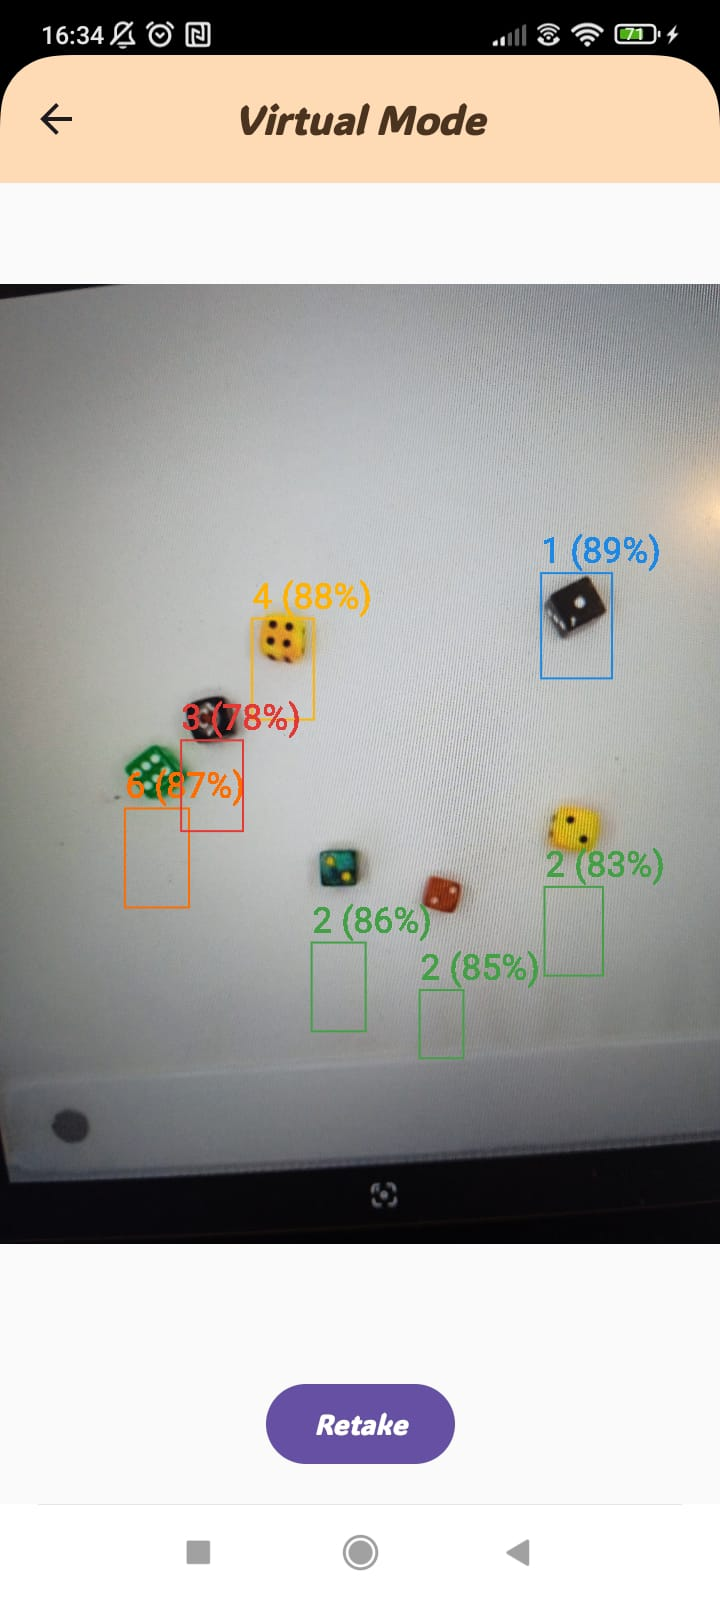
\includegraphics[width=\textwidth]{img/virtual screen.jpg}
    \end{subfigure}
    \hfill
    \begin{subfigure}[b]{0.27\textwidth}
        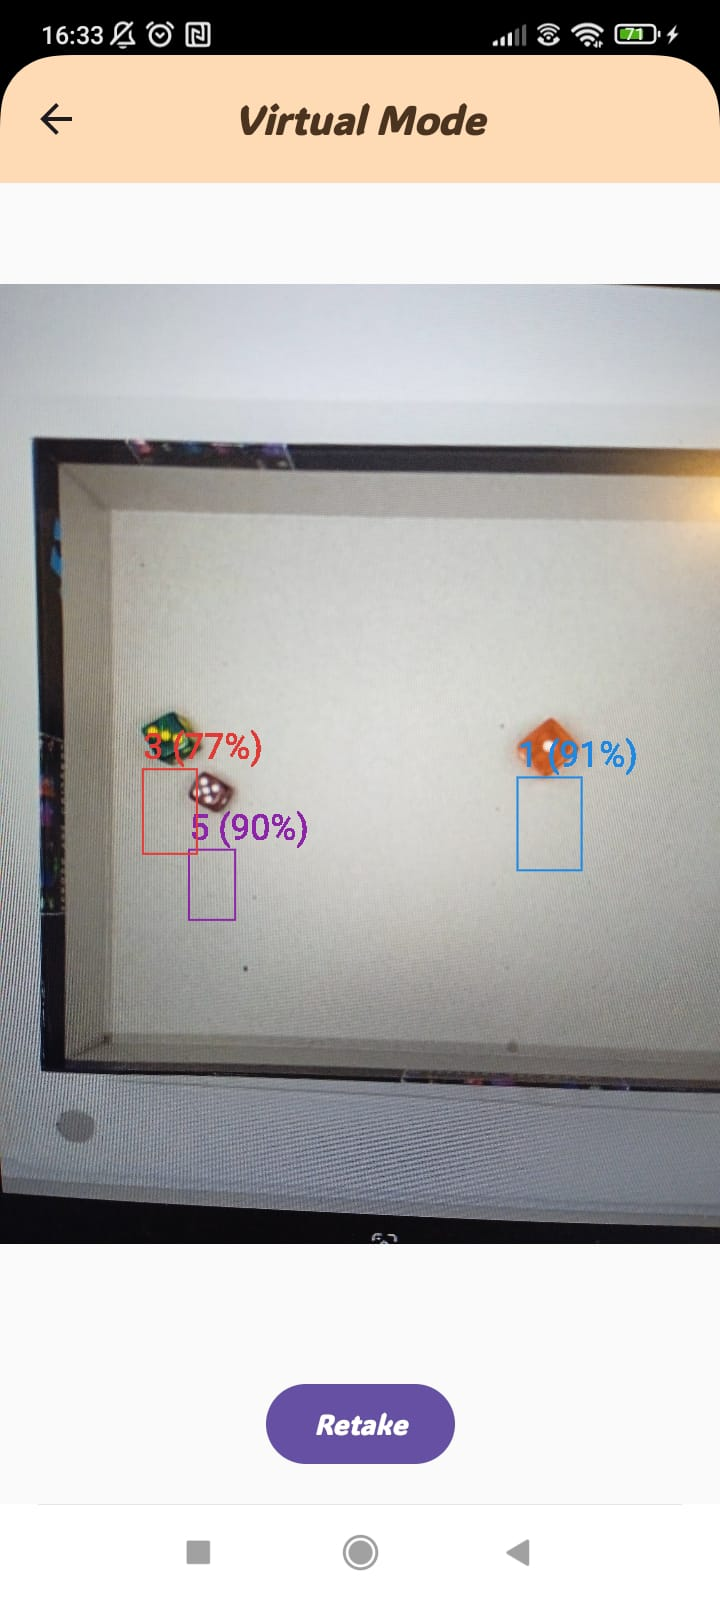
\includegraphics[width=\textwidth]{img/virtual screen2.jpg}
    \end{subfigure}
    \hfill
    \begin{subfigure}[b]{0.27\textwidth}
        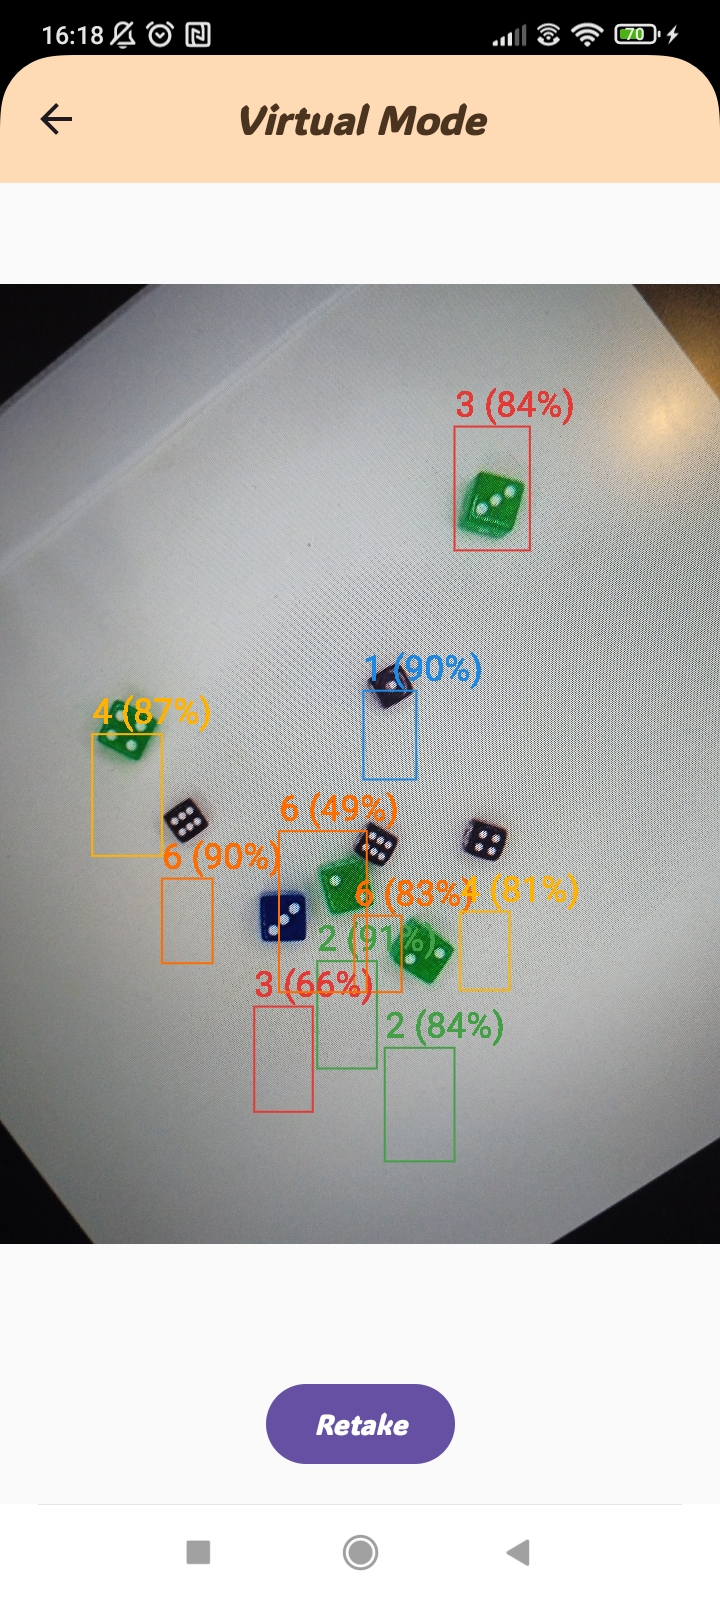
\includegraphics[width=\textwidth]{img/virtual screen3.jpg}
    \end{subfigure}   
    \caption{Image Recognition of Dice.}
    \label{fig:image_recognition}
\end{figure}


\begin{figure}[ht!]
    \centering
    \begin{subfigure}[b]{0.26\textwidth}
        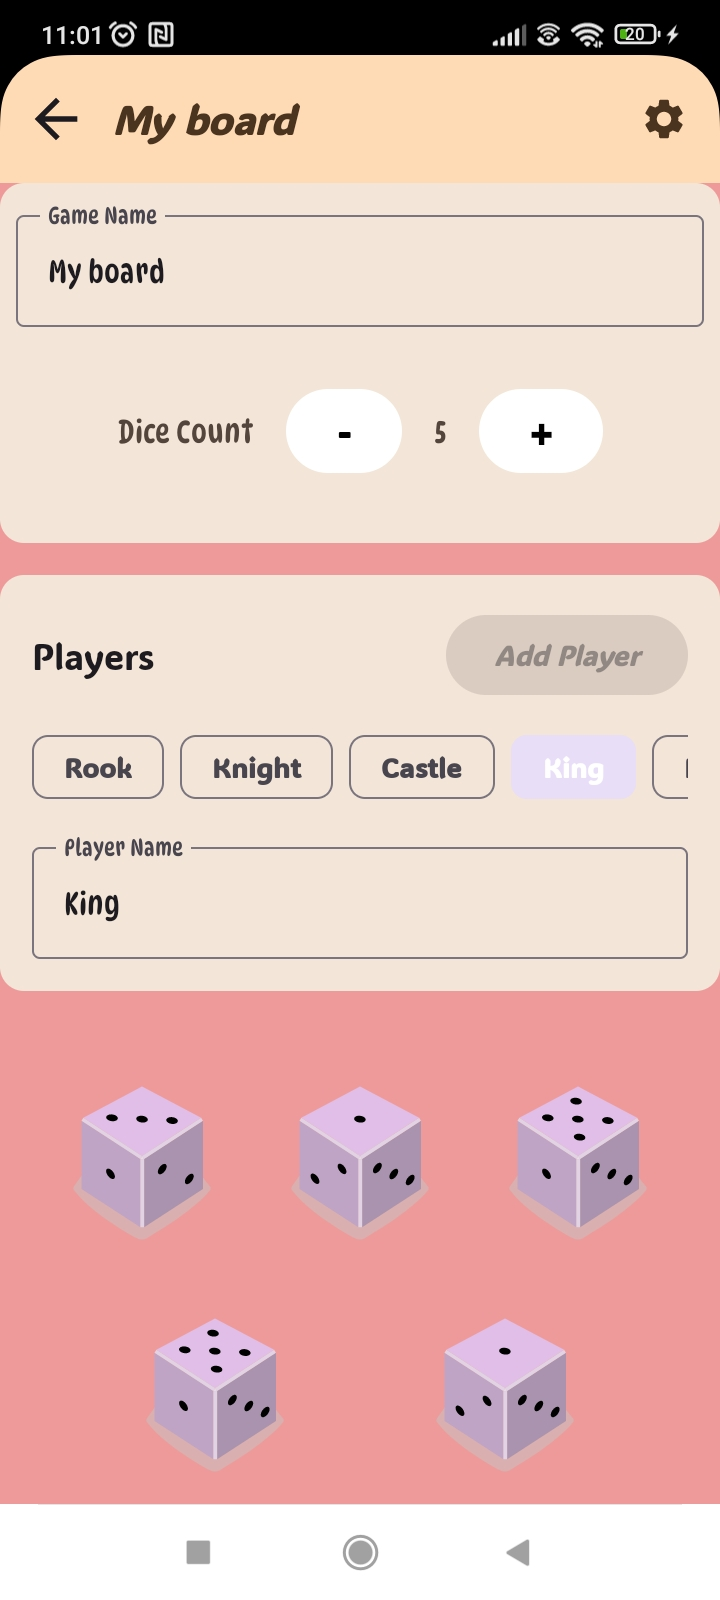
\includegraphics[width=\textwidth]{img/custom game2.jpg}
    \end{subfigure} 
    \hspace{.5em}
    \begin{subfigure}[b]{0.26\textwidth}
        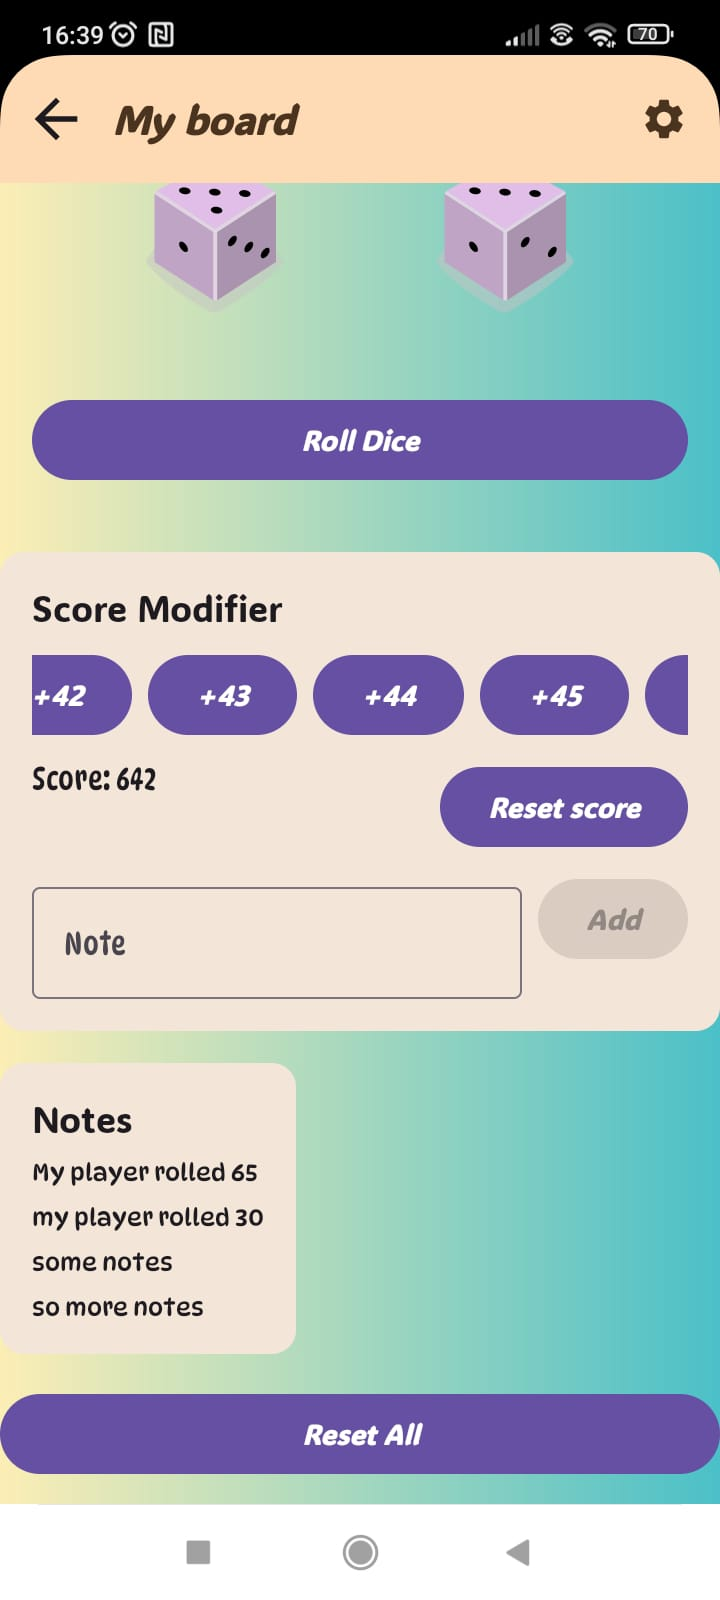
\includegraphics[width=\textwidth]{img/custom game.jpg}
    \end{subfigure}
    \caption{Custom Game Board allowing users to personalize their game settings}
    \label{fig:custom_game_board}
\end{figure}

\begin{figure}[ht!]
    % \centering
    \begin{subfigure}[b]{0.27\textwidth}
        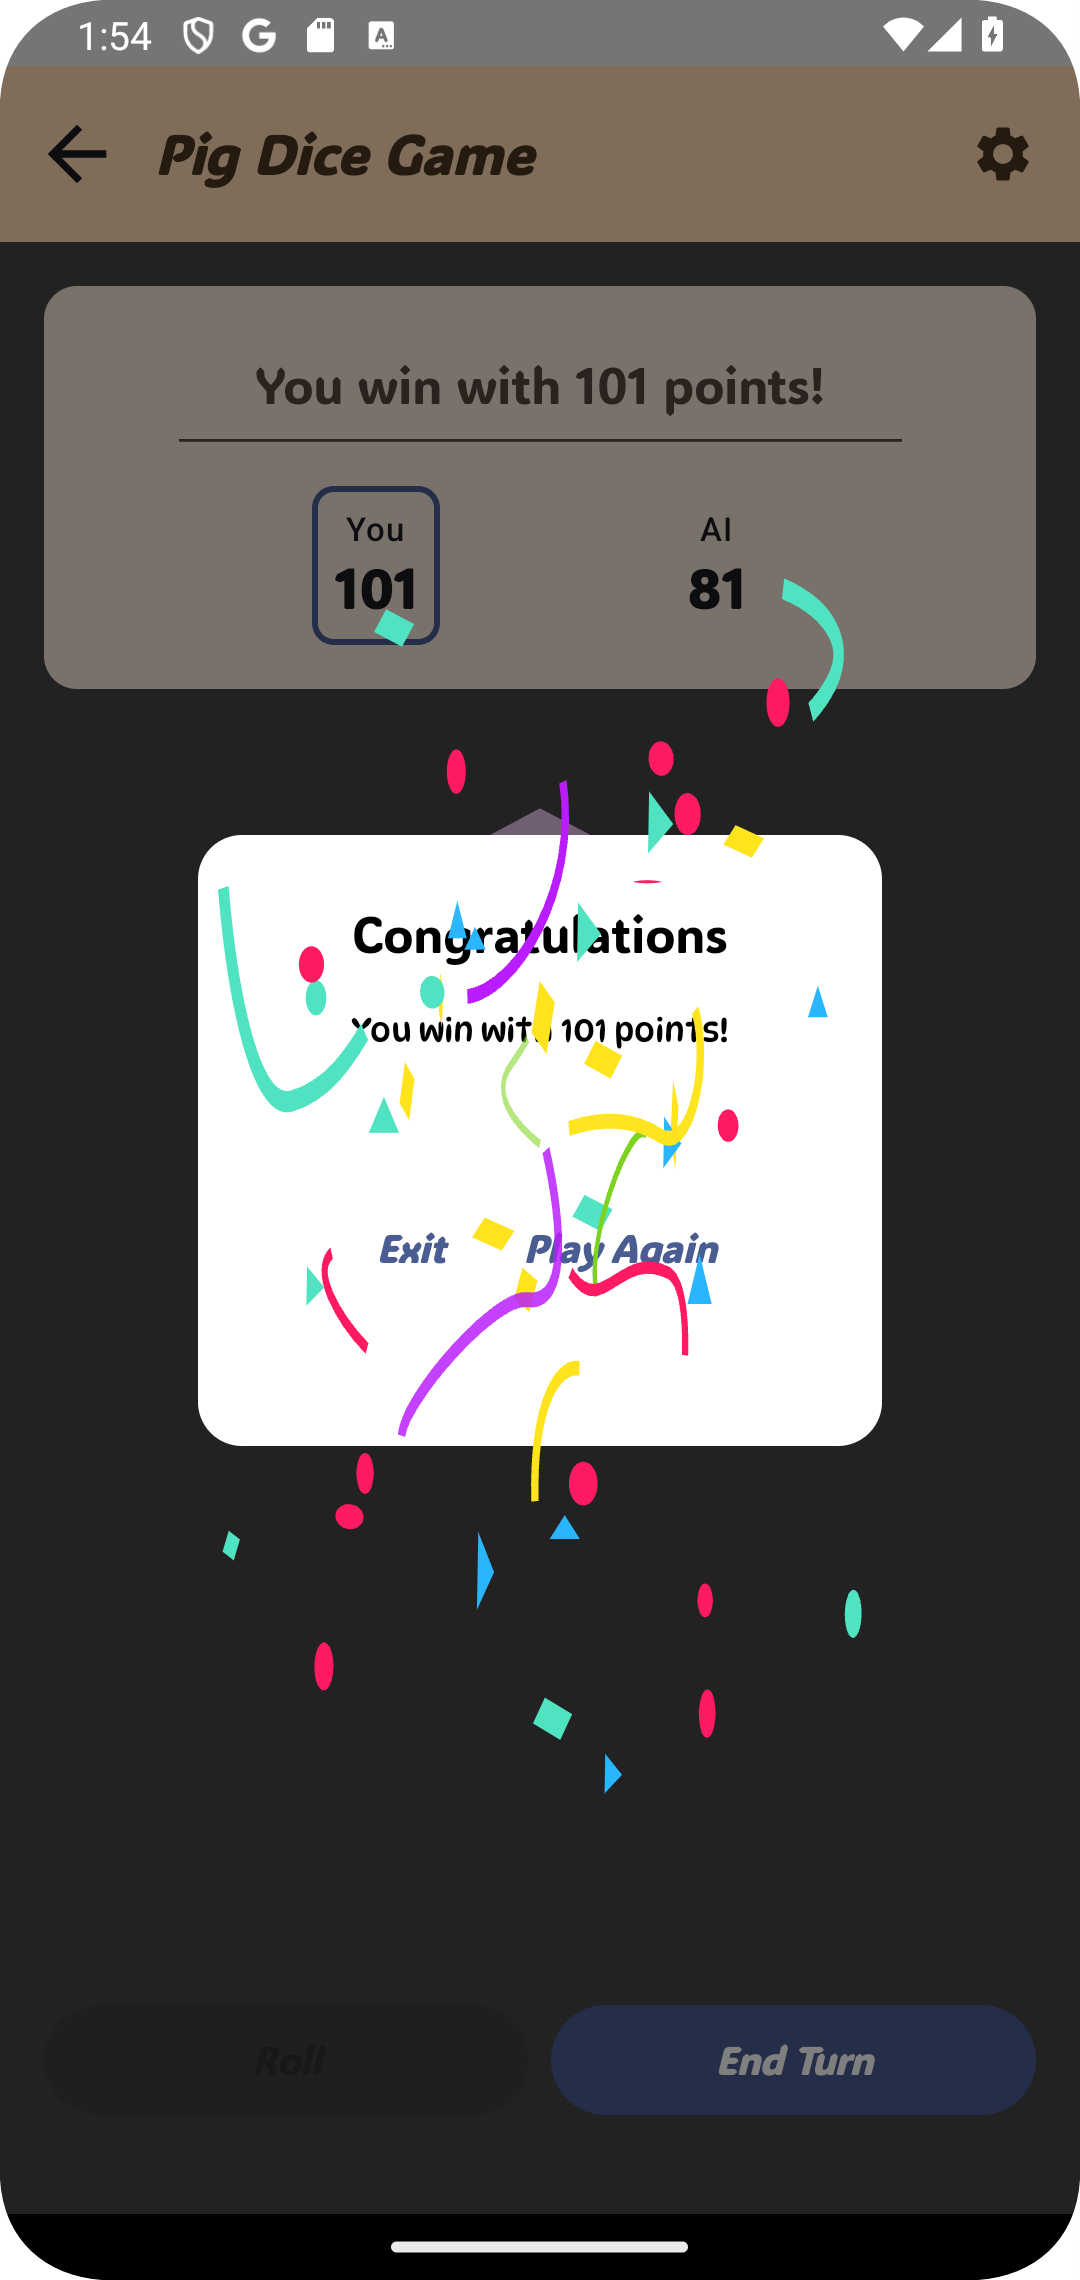
\includegraphics[width=\textwidth]{img/pig board3.png}
        \caption{Winning a Game of Pig with the final score displayed on the board}
    \end{subfigure}
    \hfill
    \begin{subfigure}[b]{0.27\textwidth}
        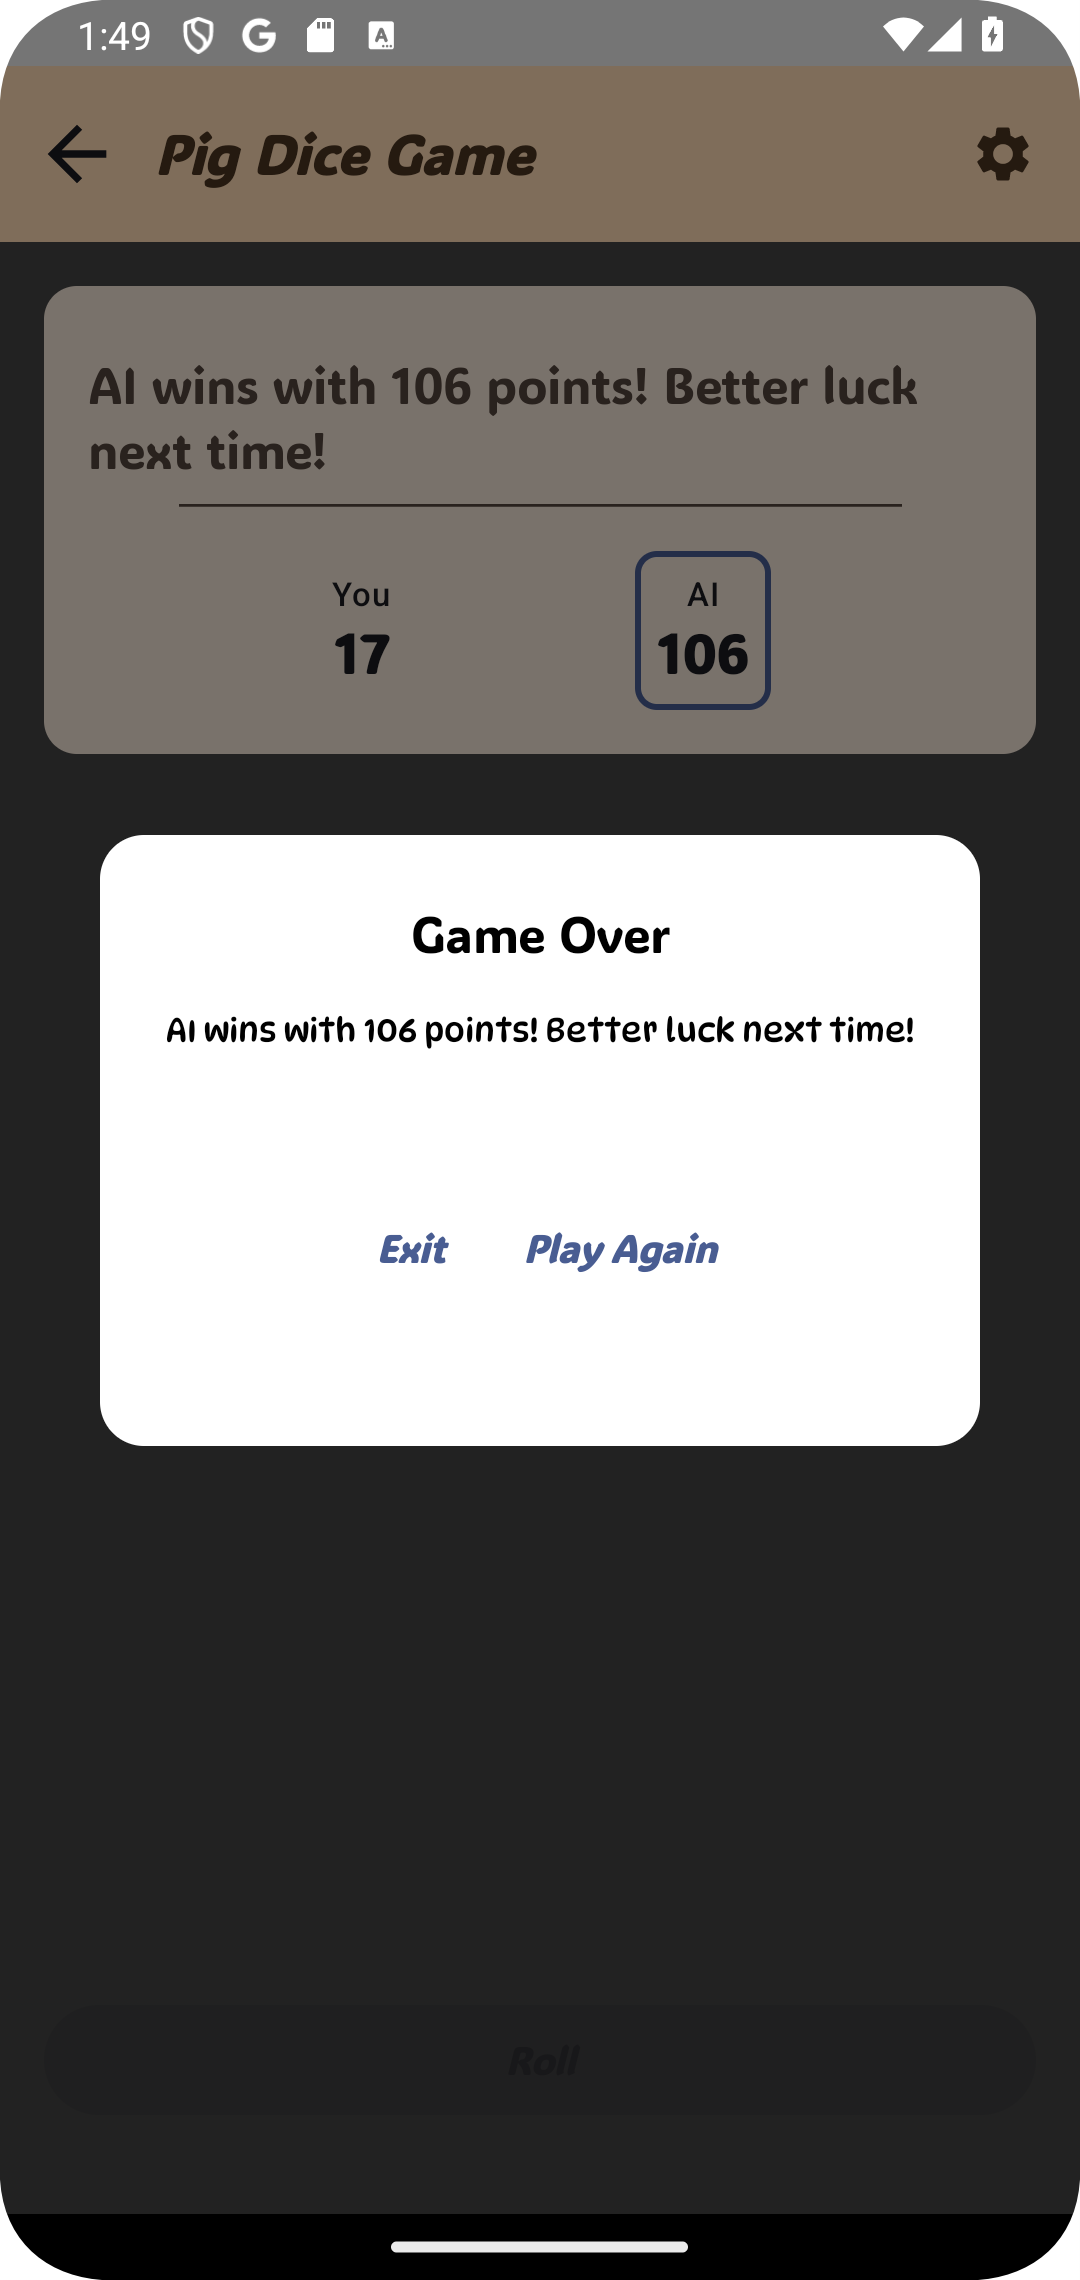
\includegraphics[width=\textwidth]{img/pig board2.png}
        \caption{Losing a Game of Pig, showing the end game scenario}
    \end{subfigure}
    \hfill
    \begin{subfigure}[b]{0.27\textwidth}
        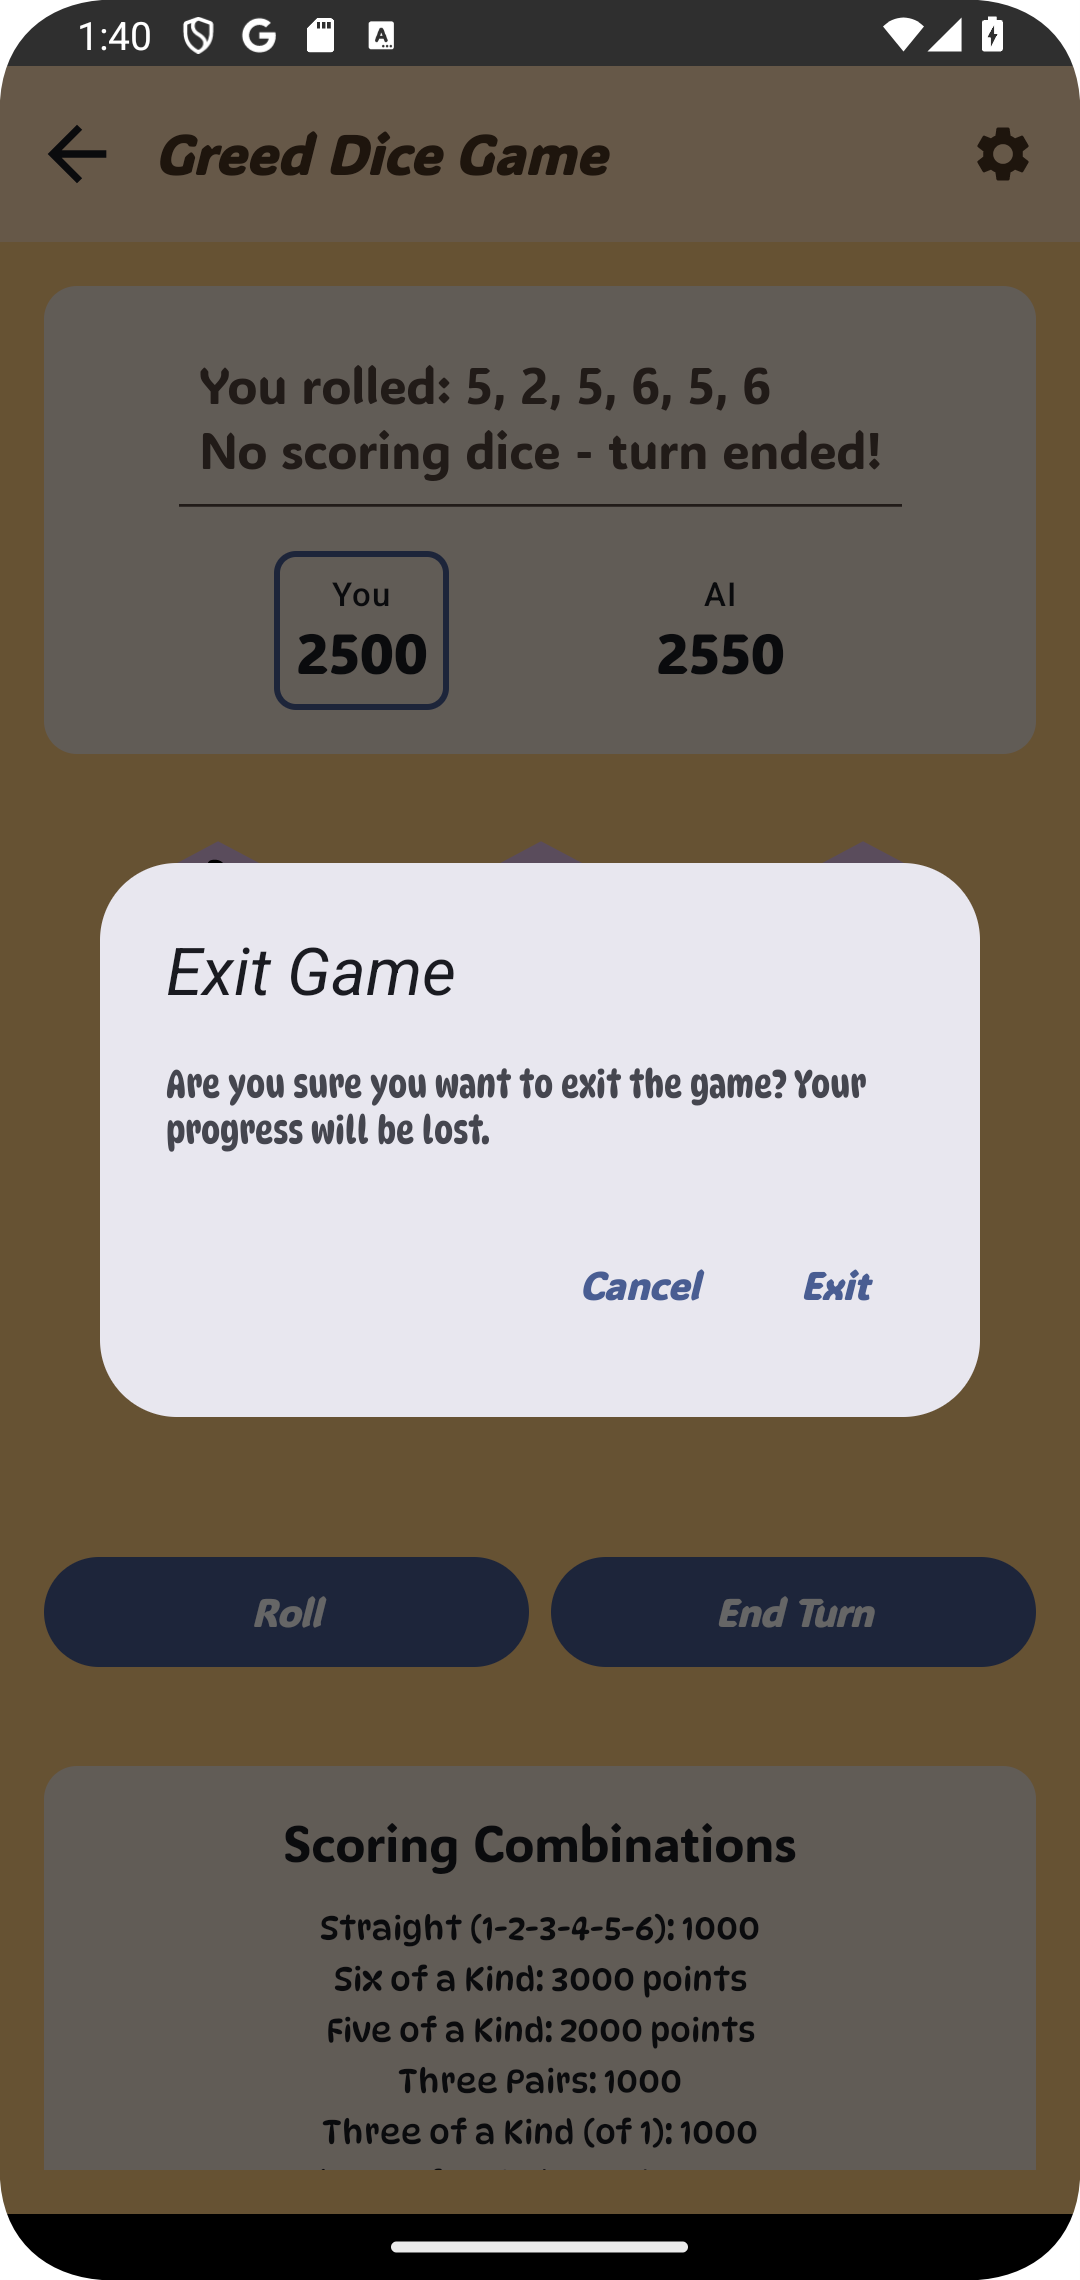
\includegraphics[width=\textwidth]{img/greed board2.png}
        \caption{Exiting a game of Greed after finalizing the score}
    \end{subfigure}
    \caption{Board Features and Game Scenarios}
    \label{fig:additional_features}
\end{figure}
